\chapter{\whatIsTitle?}\label{warmup}


Many difficult problems can be handled easily 
once  relevant information is organized in a certain way. 
This text aims to teach you how to organize information in cases where certain mathematical structures are present. 
Linear algebra is, in general, the study of those structures. Namely

\vspace{3mm}
\shabox{Linear algebra is the study of vectors and linear functions.} 
\vspace{3mm}

\noindent In broad terms, vectors are things you can add and  linear functions are %very special 
functions of vectors that respect vector addition. 
The goal of this text is to teach you to organize information about vector spaces in a way that makes problems involving linear functions of many variables easy. 
(Or at least tractable.) 

To get a feel for the general idea of organizing information, of vectors, and of linear functions this chapter has brief sections on each. 
We start here in hopes of putting students in the right mindset for the 
odyssey that follows; the latter chapters cover the same material at a slower pace.  
% a little better lets try some examples. 
Please be prepared to change the way you think about some familiar mathematical objects
and keep a pencil and piece of paper handy!

\section{Organizing Information}
\label{organize}
Functions of several variables are often presented in one line such as 
\[f(x,y)=3x+5y\,.\]
But lets think carefully; what is the left hand side of this equation doing? 
Functions and equations are different mathematical objects so why is the equal sign necessary?

\begin{center}
\href{https://www.youtube.com/watch?v=dvoG5P9Uczg}{\raisebox{-.4cm}{
\includegraphics[scale=.075]{take1.jpg}}} \hspace{1cm}\scalebox{1.2}{\tt A Sophisticated Review of Functions }
\end{center}
If someone says 
\vspace{-.01cm}
\begin{center}
``Consider the function of two variables $7\beta-13 b$." 
\end{center}
we do not quite have all the information we need to determine the relationship between inputs and outputs. 
%This is the foundation of the powerful yet easy to use  mathematics known as linear algebra. 
%%%%an alternative wording
%Difficult %science 
%problems involving multiple variables can be handled easily 
%once  relevant information is organized in a certain way. 
%You are about to learn powerful methods of organizing information 
%applicable when a certain kind of  object is involved in a problem; a linear function. It takes quite a bit of work to understand what a linear function is, but it does not take much to see what it looks like to organize information.   
%%This is the foundation of the powerful yet easy to use  mathematics known as linear algebra. 
\begin{example} (Of organizing and reorganizing information)\\ \label{OrderInfo}
You own stock in 3 companies: $Google$, $Netflix$, and $Apple$. 
The value $V$ of your stock portfolio as a function of the number of shares you own $s_{N}, s_{G},s_{A}$ of these companies 
%with logos 
 is %given by
\[
%%%%%%%%%%%%%%%%
%%%% HEY 
%%%% Do not type V\colvec{ s_a\\s_b\\s_c }= here!
%%%%That already involves choice of  an order! 
24s_{G}+80s_{A}+35s_{N}\,.\]
Here is an ill posed question: what is $V\colvec{1\\2\\3} $?\\

The column of three numbers is ambiguous! 
%We can't determine if 
Is it is meant to denote % the value of your portfolio 
\begin{itemize}
\item 1 share of ${G}$, 2 shares of ${N}$ and 3 shares of ${A}$? 
\item 1 share of ${N}$, 2 shares of ${G}$ and 3 shares of ${A}$?  
\end{itemize}
Do we multiply the first number of the input by 24 or by 35? 
No one has specified an order for the variables, 
so we do not know how to calculate an output associated with a particular input.\!\footnote{Of course we would know how to calculate an output if the input is described in the tedious form such as ``1 share of ${G}$, 2 shares of ${N}$ and 3 shares of ${A}$", but that is unacceptably tedious! We want to use ordered triples of numbers to concisely describe inputs.}% that input is written as a triple of numbers. 

A different notation for $V$ can clear this up; 
%since specifying an oder for the variables amounts to instructions of which number from the input to multiply by which of thee numbers 80, 35, 24, 
we can denote $V$ itself as an ordered triple of numbers that reminds 
us what to do to each number from the input.
\begin{center}
\shabox{Denote $V$ by  $\rowvec{ 24 &80& 35 } $ and thus write 
$V\colvec{ 1\\2\\3 }_{\!\!\!\!B }
= 
\begin{pmatrix} 24 &80& 35 \end{pmatrix}
\colvec{ 1\\2\\3 }%_{\!\!\! \!\alpha }.
$
\qquad \qquad
\phantom{ $\colvec{1\\2} $}%for space
to remind us to calculate 
$24(1)+80(2)+35(3)=334$ \qquad\qquad
\phantom{ $\colvec{1\\2} $}%for space
because we chose the order 
%$\colvec{s_{G}\\s_ {A}\\s_{N}}$ 
$\colvec{{G} & {A} & {N}}$ 
and named that order $B$ \qquad
so that inputs are interpreted as 
$\colvec{s_{G}\\s_ {A}\\s_{N}}$ 
.} 
\end{center}
%as a concise reminder of how to calculate the output assigned to any particular input ... {\itshape but only if you know what the input means}. 
%The input is a column of three numbers. 
%You need to know to interpret the 
%top number as stock in company $a$, 
%second from the top in company $b$, etc.. 
%Thus, the choice of notation for $V$ involved a choice of order of the companies. 
If we change the order for the variables we should change the notation for $V$.
\begin{center}
\shabox{
Denote $V$ by  $\rowvec{  35 & 80& 24 } $ and thus write 
$V\colvec{ 1\\2\\3 }_{\!\!\!\!B'}
= 
\rowvec{  35 & 80& 24 } 
\colvec{ 1\\2\\3 }$
\qquad \qquad
\phantom{ $\colvec{1\\2} $}%for space
to remind us to calculate 
$35(1)+80(2)+24(3) =264.$ \qquad\qquad
\phantom{ $\colvec{1\\2} $}%for space
because we chose the order 
$\colvec{{N} & {A} & {G} }$ 
and named that order $B'$\qquad
so that inputs are interpreted as 
$\colvec{s_{N}\\ s_ {A}\\ s_{G}}$ 
.
} 
\end{center}
The  subscripts $B$ and $B'$ on the columns of numbers are just symbols\footnote{We were free to choose any symbol to denote these orders. We chose $B$ and $B'$ because we are hinting at a central idea in the course: choosing a basis.} reminding us of how to interpret the column of numbers.
But the distinction is critical; as shown above
$V$ assigns completely different numbers to the same  columns of numbers with different subscripts. 

There are six different ways to order the three companies. 
Each way will give different notation for the same function $V$, and a different way of assigning numbers to columns of three numbers. 
Thus, it is critical to make clear which ordering is used if the reader is to understand what is written. 
Doing so is a way of organizing information. 

This example is a hint at a much bigger idea central to the text; 
our choice of order is an example of choosing a {\itshape basis}\footnote{
Please note that this is an {\itshape example} of choosing a basis, 
not a statement of the definition of the technical term ``basis". 
You can no more learn the definition of ``basis"  from this example 
than learn the definition of  ``bird" by seeing a penguin.}\!\!. 
\end{example}

The main lesson of an introductory linear algebra course is this: 
you have considerable freedom in how you organize information about certain functions, 
and you can use that  freedom to 
\begin{enumerate}
\item uncover aspects of functions that don't change with the choice (Ch \ref{eigenvalseigenvects})
\item make calculations maximally easy (Ch \ref{sec:diagonalization}  and Ch \ref{sec:leastsquaresSVD}) 
\item approximate functions of several variables (Ch \ref{sec:leastsquaresSVD}).
\end{enumerate}
Unfortunately, because the subject (at least for those learning it) requires seemingly arcane and tedious computations
involving large arrays of numbers known as matrices, the key concepts and the wide applicability of linear algebra are
easily missed. So we reiterate, 

\vspace{3mm}
\shabox{Linear algebra is the study of vectors and linear functions.} 
\vspace{3mm}

\noindent In broad terms, vectors are things you can add and  linear functions are 
functions of vectors that respect vector addition. 


%%%%%%%%%%%%%%%%%%%%%%%%%%%%%%%%
%%%%%%%%%%%%%%%%%%%%%%%%%%%%%%%%

%\newpage
\noindent 
\section{What are Vectors?}
Here are some examples of things that can be added:

\begin{example} (Vector Addition)
\begin{enumext}[label=\Alph*,wrap-label=(#1)]
\item Numbers: Both $3$ and $5$ are numbers and so is $3+5$.\\[-2mm]
\item 3-vectors: $\colvec{1 \\ 1\\ 0} + \colvec{0\\1\\1}=\colvec{1 \\ 2\\ 1}$.\\[-1mm]
\item Polynomials: If $p(x)=1+x-2x^2+3x^3$ and $q(x)=x+3x^2-3x^3+x^4$ then\\[1mm] their sum $p(x)+q(x)$ is the new polynomial $1+2x+x^2+x^4$.\\
\item Power series: If $f(x)=1+x+\frac1{2!} x^2 + \frac1{3!} x^3 +\cdots$ and $g(x)=1-x+\frac1{2!} x^2 - \frac1{3!} x^3 +\cdots$ \\[1mm]
 then $f(x)+g(x)=2+ x^2 +\frac2 {4!} x^4+\cdots$ is also a power series.\\
\item Functions: If $f(x)=e^x$ and $g(x)=e^{-x}$ then their sum $f(x)+g(x)$ is the new function $2\cosh x$.
\end{enumext}
\end{example}

\noindent
There are clearly different kinds of vectors. 
Stacks of numbers are not the only things that are vectors, as examples C, D, and E show. 
Vectors of different kinds can not be added; What possible meaning could the following have? 
\[\colvec{9\\3} + e^x\]

In fact, you should think of all five kinds of vectors above as different kinds, and that you should not add vectors that are not of the same kind. 
On the other hand, any two things of the same kind ``can be added''. 
This is the reason you should now start thinking of all the above objects as vectors! 

In Chapter~\ref{vectorSpaces} we will give the precise rules that  vector addition must obey. 
In the above examples, however, notice that the vector addition rule stems from the rules for adding numbers. 
 

When adding the same vector over and over, for example
\[
x+x\, ,\: \  x+x+x\, ,\:\    x+x+x+x\,  ,\, \ldots\, ,
\]
we will write
\[
2x\, ,\: \, 3x\, , \:\,  4x\, ,\, \ldots\, ,
\]
respectively. For example
\[
4\colvec{1\\1\\0}=\colvec{1\\1\\0}+\colvec{1\\1\\0}+\colvec{1\\1\\0}+\colvec{1\\1\\0}=\colvec{4\\4\\0}\, .
\]
Defining $4x=x+x+x+x$ is fine for integer multiples, but does not help us make sense of $\frac13 x$. For the different types of vectors 
above, you can probably guess how to multiply a vector by a scalar. For example
\[
\frac 13 \colvec{1\\[1mm]1\\[1mm]0} = \colvec{\frac13\\[1mm] \frac13\\[1mm]0}\, .
\]

 A very special vector can be produced from any vector of any kind by scalar multiplying any vector by the number~$0$. 
This is called the {\itshape zero vector}\index{Zero vector} and is usually denoted simply $0$. This gives five very different kinds of zero from the 5 different kinds of vectors in   examples A-E above.
\begin{enumext}[label=\Alph*,wrap-label=(#1)]
\item $0(3)=0$ (The zero number)
\item $0\colvec{1\\1\\0}=\colvec{0\\0\\0} $ (The zero 3-vector)
\item $0\left(1+x-2x^2+3x^3\right)=0$ (The zero polynomial)
\item 
$0\!\left(  1+x\!-\!\frac1{2!}x^2\!+\!\frac1{3!}x^3\!+\cdots \!\right) \!
 =  0+0x+0x^2\!+0x^3\!+\cdots $(The zero power~series)
 \item $0\left(   e^x \right) =0$ (The zero function)
\end{enumext}

In any given situation that you plan to describe using vectors, you need to decide on a way to add and scalar multiply vectors.
In summary:
\vspace{3mm}
\begin{center}
\shabox{Vectors are things you can add and scalar multiply.} 
\end{center}
\vspace{3mm}

\noindent 
Examples of kinds of vectors:\\
\begin{itemize}
\item numbers
\item n-vectors
\item 2nd order polynomials
\item polynomials
\item power series
\item functions with a certain domain
\end{itemize}



\section{What are Linear Functions?}
\label{LTs}

In calculus classes, the main subject of investigation was the rates of change of functions. 
In linear algebra, functions
will again be the focus of your attention, 
but functions of a very special type. 
In precalculus you 
were perhaps encouraged to think of a function as a machine~$f$
into which one may feed a real number. 
For each input $x$ this machine outputs a single real number~$f(x)$. 

\begin{center}
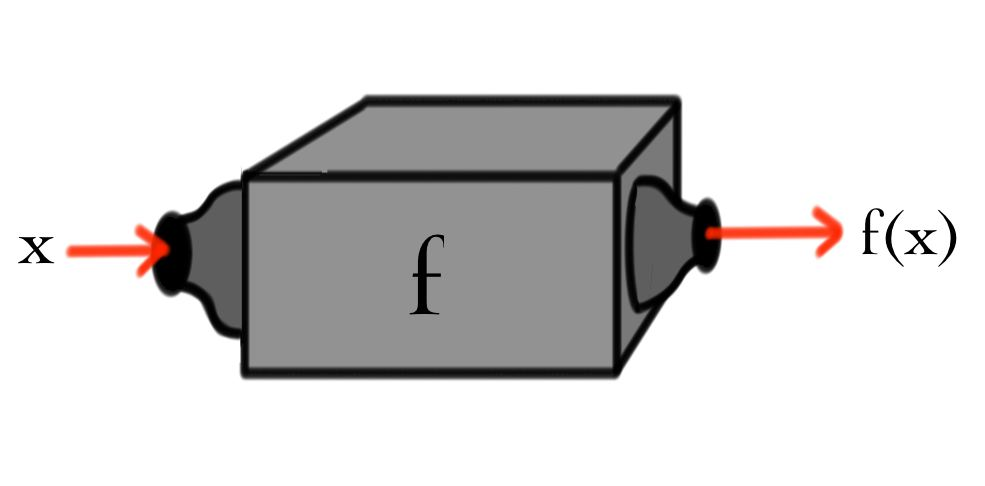
\includegraphics[scale=.3]{\whatIsPath//machine.jpg}
\end{center}

In linear algebra, the functions we study will have vectors (of some type) as both inputs and outputs. 
We just saw that vectors are objects that can be added or scalar multiplied---a very general notion---so the functions we are going to study will look novel at first. 
So things don't get too abstract, here are five questions that can be rephrased in terms of functions of vectors.

\begin{example}  \label{EX}
(Questions involving Functions of Vectors in Disguise)\\
\begin{enumext}[label=\Alph*,wrap-label=(#1)]
\item\label{FVA}What number $x$ satisfies $10x=3$?
\item\label{FVB} What 3-vector~$u\!\, $  satisfies\footnote{ The \hyperlink{crossprod}{cross product} appears in this equation.}~$\!\colvec{1 \\ 1\\ 0} \times u = \colvec{0\\1\\1}$?\\[-.4cm]
%\[\!\!\!\!\!\!\!\!\!\colvec{x\\ y\\ z} \raisebox{-11mm}{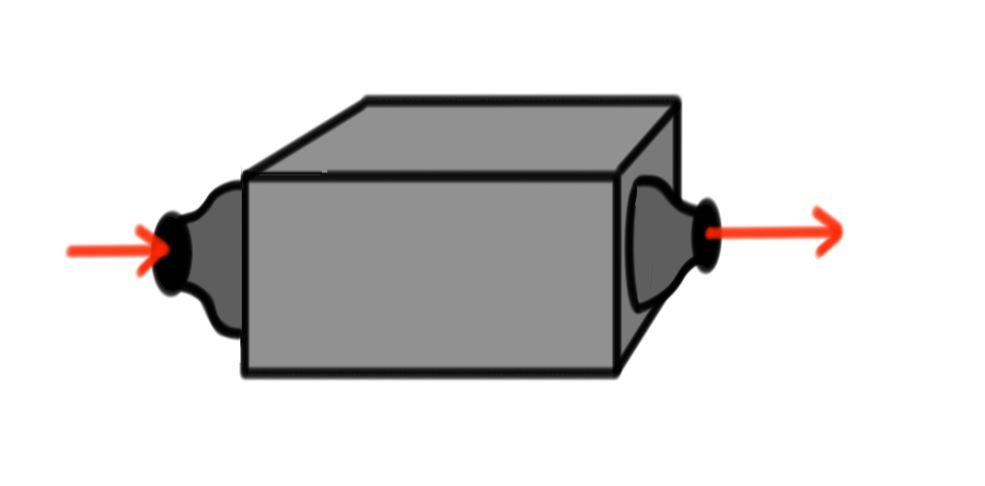
\includegraphics[scale=.14]{\whatIsPath//machine_blank.jpg} }\! \! \!\! \! \!\colvec{\phantom{-}z\\-z\\y-x}\]
\item \label{FVC}What polynomial~$p$ satisfies~$\int_{-1}^1  p(y) dy = 0$ and $\int_{-1}^1 y p(y) dy=1$?\\
%\[p(x) \raisebox{-11mm}{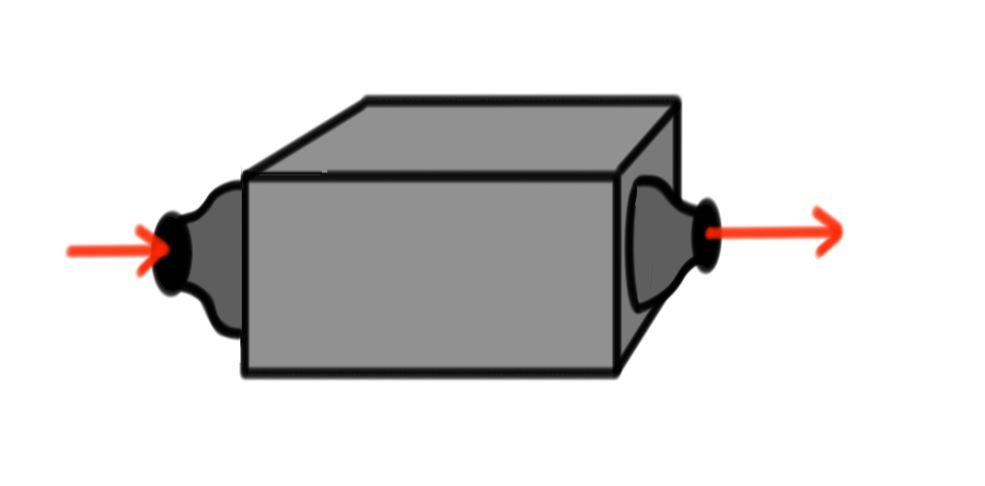
\includegraphics[scale=.14]{\whatIsPath//machine_blank.jpg} }\! \! \!\! \! \!\colvec{\int_{-1}^1  p(y) dy\\[2mm]
%x\int_{-1}^1 y p(y) dy}\]
\item \label{FVD}What power series~$f(x)$ satisfies~$x\frac{d}{dx} f(x) -2f(x)=0$?
%\[f(x) \raisebox{-11mm}{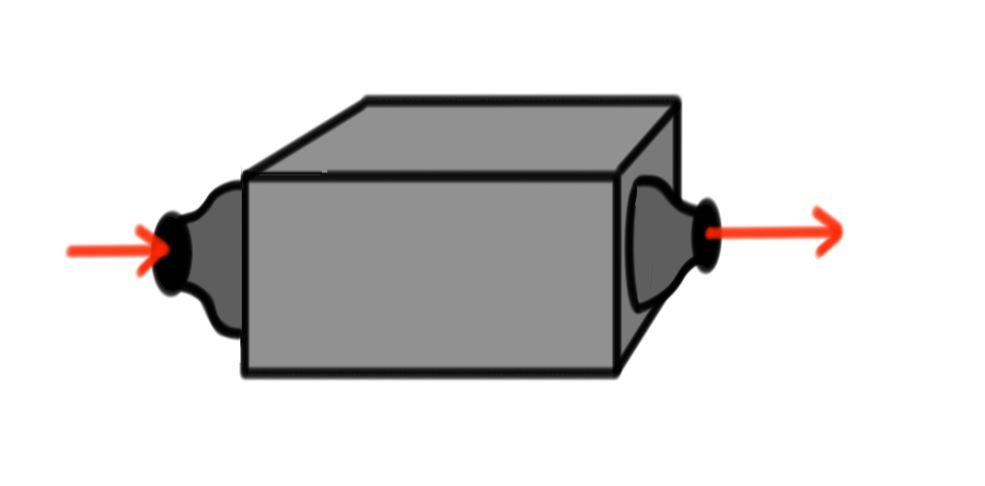
\includegraphics[scale=.14]{\whatIsPath//machine_blank.jpg} }\! \! \!\! \! \!x\frac{d}{dx} f(x) -2f(x)\]
\item What number~$x$~satisfies~$4 x^2=1$?
%\[f(x) \raisebox{-11mm}{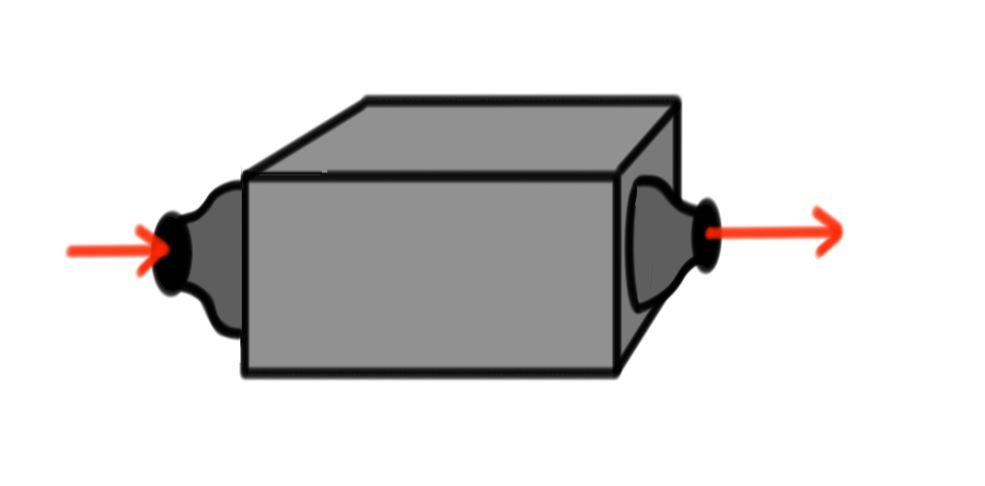
\includegraphics[scale=.14]{\whatIsPath//machine_blank.jpg} }\! \! \!\! \! \!f''(x)+f^3(x) -\sqrt{x}\]
\end{enumext}
\vspace{.3cm}
All of these are of the form 
\begin{itemize}
\item[($\star$)] What vector $X$ satisfies $f(X)=B$?
\end{itemize}
with a function\footnote{In math terminology, each question is asking for the level set of $f$ corresponding to $B$.} $f$ known, a vector $B$ known, and a vector $X$ unknown.
\end{example}
The machine needed for part~(\ref{FVA}) is as in the picture below. 
\[x \raisebox{-11mm}{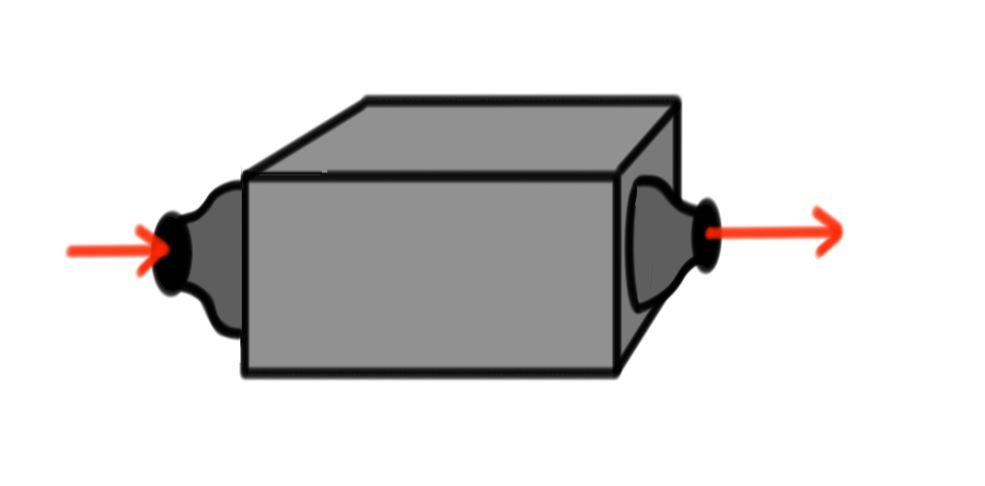
\includegraphics[scale=.14]{\whatIsPath//machine_blank.jpg} }\! \! \!\! \! \!10 x\, \hspace{8mm}\]
This is just like a function $f$ from calculus that takes in a number $x$ and spits out the number $10x$. (You might write $f(x)=10x$ to indicate this).
For part~(\ref{FVB}), we need something more sophisticated. 
\[\!\!\!\!\!\!\!\!\!\colvec{x\\ y\\ z} \raisebox{-11mm}{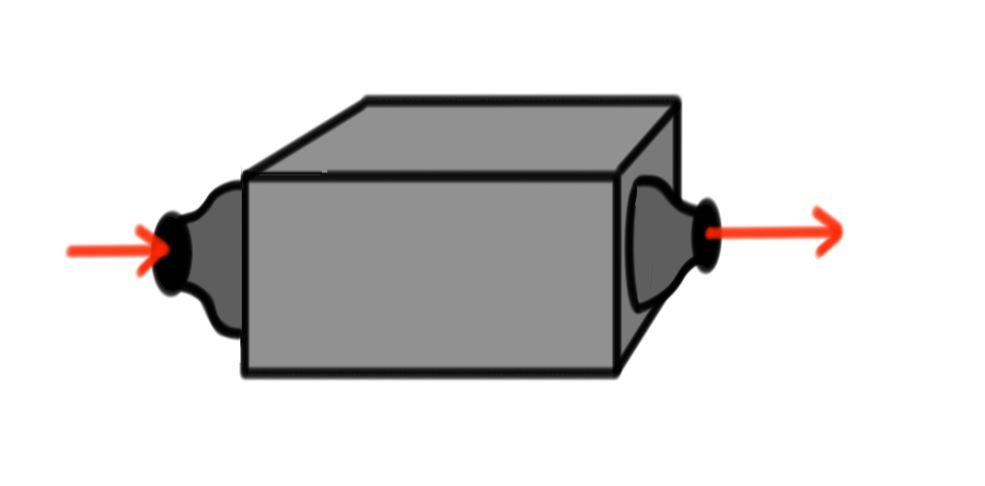
\includegraphics[scale=.14]{\whatIsPath//machine_blank.jpg} }\! \! \!\! \! \!\ccolvec{\phantom{-}z\\-z\\\!y-x\!\!}\, ,\]
The inputs and outputs are both 3-vectors. The output is the cross product of the input with... how about you complete this sentence to make sure you understand.

The machine needed for example~(\ref{FVC}) looks like it has just one input and two outputs; we input a polynomial and get a 2-vector as output.
\[\quad p \raisebox{-11mm}{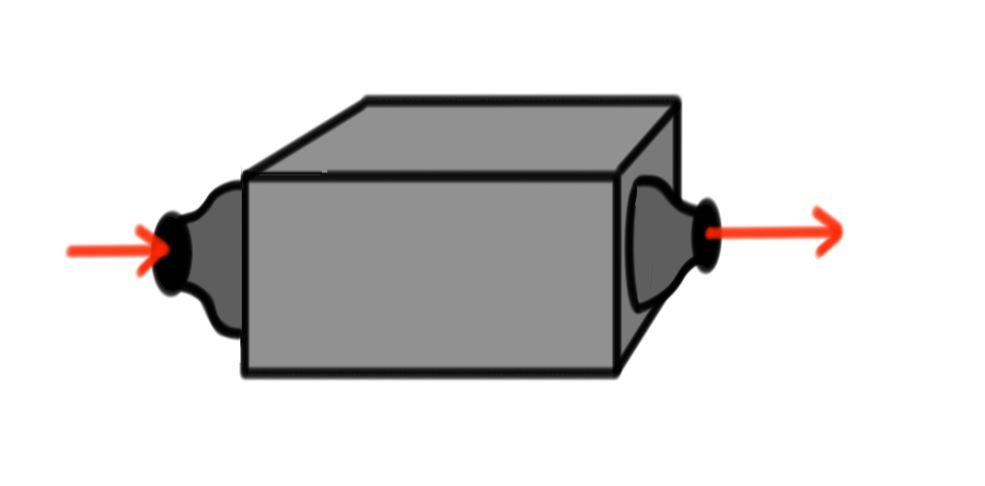
\includegraphics[scale=.14]{\whatIsPath//machine_blank.jpg} }\! \! \!\! \! \!\colvec{\int_{-1}^1  p(y) dy\\[3mm]
\int_{-1}^1 y p(y) dy}\, .\]
This example is important because it displays an important feature; 
{\itshape the inputs for this function are functions}.

While this sounds complicated, %Rest assured that 
linear algebra is the
%involves the 
study of %only a very 
simple %(yet very important) class of 
functions of vectors; its time to describe the essential characteristics of linear functions. 

Let's use the letter $L$ to denote an arbitrary linear function and think again about vector addition and scalar multiplication. 
Also,  suppose that $v$ and $u$ are vectors and $c$ is a number. 
Since $L$ is a function from vectors to vectors, if we input $u$ into $L$, the output $L(u)$ will also be some sort of vector. 
The same goes for 
$L(v)$.
(And remember, our input and output vectors might be something other than stacks of numbers!) 
Because vectors are things that can be added and scalar multiplied, 
$u+v$ and $cu$ are also vectors, and so they can be used as inputs.
The essential characteristic of linear functions is what can be said about 
%the outputs 
$L(u+v)$ and $L(cu)$ in terms of 
%the outputs 
$L(u)$ and $L(v)$. 

Before we tell you this essential characteristic, 
ruminate on this picture. 

\begin{center}
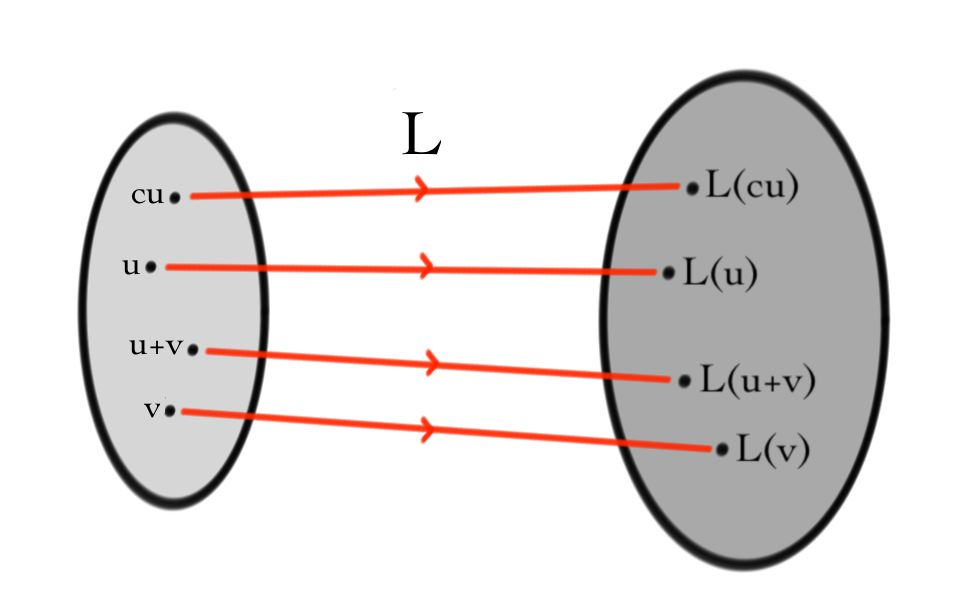
\includegraphics[scale=.4]{\whatIsPath/L.jpg}
\end{center}

The ``blob'' on the left represents all the vectors that you are allowed to input into the function $L$,  the blob on the right denotes the
possible outputs, and the lines tell you which inputs are turned into which outputs.\footnote{The domain, codomain, and rule of correspondence of the function are represented by the left blog, right blob, and arrows, respectively.} A full pictorial description of the functions would require all inputs and outputs and lines to be explicitly drawn, but we are being diagrammatic; we only drew four of each.  




Now think about adding $L(u)$ and $L(v)$ to get yet another vector $L(u)+L(v)$ or of multiplying $L(u)$ by $c$ to obtain the vector $cL(u)$, and placing both on the right blob of the picture above. 
But wait! Are you certain that these are possible outputs!?
%Hopefully you noticed that there are two vectors  apparently {\itshape not shown} on the blob of outputs:
%\[
%L(u)+L(v)\quad \&\quad cL(u)\, .
%\] 
%You might already be able to guess the values we would like these to take. If not, 

Here's the answer 
\begin{center}
\shabox{\scalebox{1.1}{
The key to the whole class, from which everything else \hypertarget{twopart}{follows}: 
%\newline The essential features of a linear function $L$ are
}}
\end{center}
\begin{enumerate}
\item Additivity:
\[L(u+v)=L(u)+L(v)\, .\]
\item Homogeneity:
\[L(cu)=cL(u)\, .\]
\end{enumerate}

\noindent Most functions of vectors do not obey this requirement.\!\footnote{{\itshape E.g.:} If $f(x)=x^2$ then $f(1+1)=4 \neq f(1)+f(1)=2$. Try any other function you can think of!}  At its heart, linear algebra is the study of functions that do. 

Notice that the additivity 
requirement says that the function $L$ respects vector addition: {\itshape it does not matter if you first add $u$ and~$v$ and then input their sum into
$L$, or first input $u$ and $v$ into $L$ separately and then add the outputs.} The same holds for scalar multiplication--try writing out the scalar multiplication version of the italicized sentence. When a function of vectors obeys the additivity and homogeneity properties we say that it is {\itshape linear} (this is the ``linear'' of linear algebra). Together, additivity and homogeneity are called {\itshape linearity}. 
Are there other, equivalent, names for linear functions? Yes:
%\begin{enumerate}[]
%\item Linear transformation 
%\item Linear map
%\item Linear operator
%\item Homomorphism
%\end{enumerate}
\begin{center}
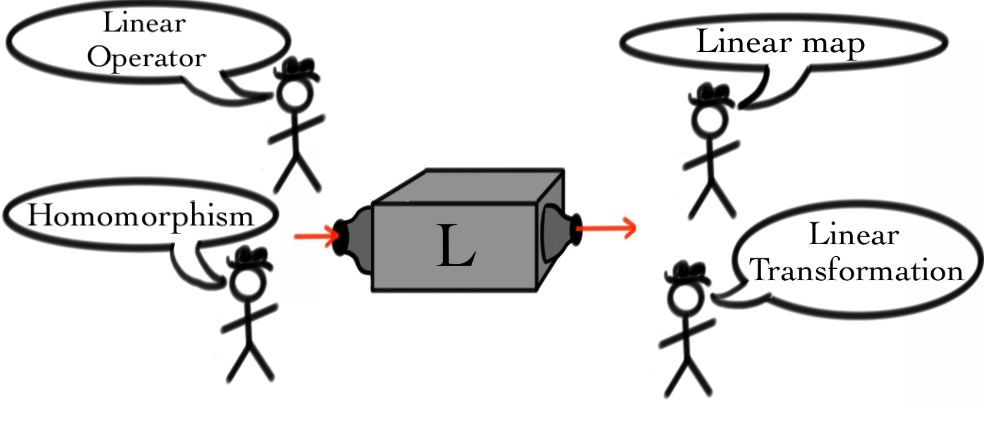
\includegraphics[scale=.37]{\whatIsPath/Names.jpg}
\\
\shabox{Function~=~Transformation~=~Operator}\\
\end{center}

And now for a hint at the power of linear algebra. 
The questions in examples~(\ref{FVA}-\ref{FVD}) can all be restated as %a single equation:
\begin{center}
\shabox{
$
L v = w
$}
\end{center}
where $v$ is an unknown, $w$ a known vector, and $L$ is  a known linear transformation.
To check that this is true, one needs to know the rules for adding vectors (both inputs and outputs)
and then check linearity of $L$. Solving the equation $Lv=w$ often amounts  to solving systems of linear equations,
the skill you will learn in  Chapter~\ref{systems}.



A great example is the derivative operator.
\begin{example} (The derivative operator is linear)\\
For any two functions~$f(x)$,~$g(x)$ and any number~$c$, in calculus you probably learnt that the derivative operator satisfies
\begin{enumerate}
\item ~$\frac{d}{dx} (cf)=c\frac{d}{dx} f$, \\[-.5cm]
\item~$\frac{d}{dx}(f+g)=\frac{d}{dx}f+\frac{d}{dx}g$.\\[-.5cm]
\end{enumerate}
If we view functions  as vectors with addition given by addition of functions and with scalar multiplication given by multiplication of functions by constants, then these familiar properties of derivatives are just the linearity property of linear maps.
\end{example}

Before introducing matrices, notice that for linear maps~$L$ we will often write simply $L u$ instead of $L(u)$. This is because the linearity
property of a linear transformation $L$ means that $L(u)$ can be thought of as multiplying the vector $u$ by the linear operator $L$.
For example, the linearity of $L$ implies that if $u,v$ are vectors and $c,d$ are numbers, then
\begin{center}
\shabox{\scalebox{1.1}{
$
L(c u + d v) = c L u + d L v\, ,
$}}
\end{center}
which feels a lot like the regular rules of algebra for numbers. Notice though, that ``$u L$'' makes no sense here.

\begin{remark}
A sum of multiples of vectors $c u + dv$ is called a {\itshape linear combination}\index{Linear combination} of $u$~and~$v$.
\end{remark}

\section{So, What is a Matrix?}
Matrices are linear functions of a certain kind. 
They appear almost ubiquitously in linear algebra because---and this is the central lesson of introductory linear algebra courses---
\begin{center}
\shabox{Matrices are the result of organizing information related to linear functions. }
\end{center}
This idea will take some time to develop, but we provided an elementary example in 
Section \ref{organize}. A good starting place to  learn about matrices is by studying {\itshape systems of  linear equations}. 

\begin{example} 
A room contains~$x$ bags and~$y$ boxes of fruit.
\begin{center}
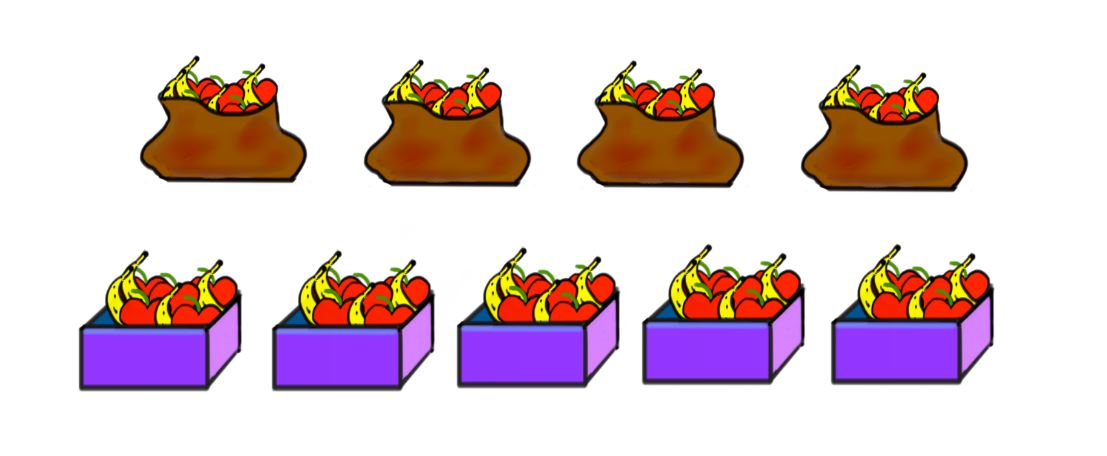
\includegraphics[scale=.25]{\whatIsPath/boxesbags.jpg}
\end{center}
Each bag contains 2 apples and 4 bananas and each box contains 6 apples and 8 bananas. 
There are 20 apples and 28 bananas in the room. Find~$x$ and~$y$.
\\

%<pic please>\\

\noindent
The values are the numbers~$x$ and~$y$ that simultaneously make both of the following equations true:
\begin{eqnarray*}
	2\, x + 6\, y & =  & 20 \\
	4\, x + 8\, y & = & 28\, .
\end{eqnarray*}
\end{example}
Here we have an example of a \emph{System of Linear Equations}\index{Linear System!concept of}.\footnote{Perhaps you can see that both lines are of the form $Lu=v$ with $u=\colvec{x\\y}$ an unknown, $v=20$ in the first line, $v=28$ in the second line, and $L$ different functions in each line? We give the typical less sophisticated description in the text above.}   
It's a collection of equations in which variables are multiplied by constants and summed, and no variables are multiplied together:  There are no powers of variables 
(like~$x^2$ or~$y^5$), non-integer or negative powers of variables (like~$y^{1/7}$ or~$x^{-3}$), and no places where variables are multiplied together (like~$xy$).
%\begin{center}\href{\webworkurl ReadingHomework1/1/}{Reading homework: problem 1.1}\end{center}
%\reading{1}{1}
\Reading{WhatIsLinearAlgebra}{1}

%The system of equations above has the feel of multiplication of contents per package by number of packages. 
%What we have is a function that takes in two numbers (number of bags and number of boxes) and gives out two numbers (number of apples and number of bananas.) 
%This function is linear: double the number of bags and the number of boxes and you will double the number of apples and number of bananas. Same for tripling, quadrupling, etc...
%
%An important idea underlies the following observation. 
\noindent
Information about the fruity contents of the room can be stored two ways: 
\begin{enumext}[label=\roman*,wrap-label=(#1)]
\item In terms of the number of apples and bananas. 
\item In terms of the number of bags and boxes. 
\end{enumext}
Intuitively, knowing the information in one form allows you to figure out the information in the other form. 
Going from~(ii) to~(i) is easy: 
If you knew there were~3 bags and~2 boxes it would be easy to calculate the number of apples and bananas, and doing so would have the feel of multiplication (containers times fruit per container). 
In the example above we are required to go the other direction, from~(i) to~(ii). This  feels like the opposite of multiplication, {\itshape i.e.}, division. Matrix notation will 
make clear what we are ``multiplying" and ``dividing'' by. 

The goal of Chapter~\ref{systems} is to efficiently solve systems of linear equations. 
%This is going to be a generalization of dividing both sides of the system of equations by...something. 
%To show you what we mean, we will now give you an example of an inefficient method of solving the system from example 3:\\
%
%\noindent
%{\bfseries Inefficient Method}:\\
%Rearrange the first equation into~$x=10-3y$ and substitute the result into the second equation to obtain~$28=4(10-3y)+8y$. This equation has only one unknown; the jargon is ``$x$ has been eliminated". The equation implies that~$y=3$. That result can be ``back substituted" into either of the original equations, for example the first, to obtain 
%$20=2x+6\cdot 3 \Leftrightarrow x=1$.\\
%
%It is easy to get lost when using this method. Especially when dealing with large systems of linear equations, such as 256 equations in 256 variables. It would be nice if we could lay out our work in a way that resonates with the intuition we have built from solving simpler algebra problems, like the familiar procedure
%\begin{eqnarray*}
%3x+4 &=&7\\
%{\rm Subtract}~&4&\\
%3x&=&3\\
%{\rm divide~by}~&3&\\
%x&=&1 \,.
%\end{eqnarray*}
%That is, lets keep the variables on the left hand side and rewrite our {\itshape system} of equations after each step. \\
%
%
%\noindent
%{\bfseries More Efficient Method:}\\
%Divide (both sides of) the second equation by 2 to obtain the equivalent system
%\begin{eqnarray*}
%	2\cdot x + 6\cdot y & = & 20 \\
%	2\cdot x + 4\cdot y  & = & 14 \,.
%\end{eqnarray*}
%Subtract the first equation from the second, to get the equivalent system 
%\begin{eqnarray*}
%	2\cdot x + 6\cdot y & =  & 20  \\
%	 0\cdot x - 2\cdot y & = & -6\, .
%\end{eqnarray*}
%Now add three times the second equation to the first
%\begin{eqnarray*}
%	2\cdot x + 0\cdot y & = & 2 \\
%	0\cdot x - 2\cdot y & = & -6\, .
%\end{eqnarray*}
%At this point the result~$x=1,y=3$ is obvious. Further, the elimination of~$y$ from the first equation and elimination of~$x$ from the second is clear as can be. 
%%This is elimination, a key idea in this course. 
%%The idea here is to follow some algorithm to have just one variable with non-zero coefficient in each equation, and to rewrite the {\itshape system} of linear equations at each step. 
%
%There is a clear shortcoming to this ``efficient method": we need to rewrite too much at each step! The~$x$'s are rewritten in the same place over and over, and similarly for the~$y$'s and the equal signs. 
%Lets work toward reducing the amount of things we rewrite by combining the pair of equations in example 3 into a singe equation using vectors from 2-space. 
Partly, this is just a matter of finding a better notation, but one that hints at a deeper underlying mathematical structure.
For that, we need rules for adding and scalar multiplying 2-vectors; 
\[
c\colvec{x\\y}:=\colvec{cx\\cy}\, \mbox{ and } \colvec{x\\y}+\colvec{x'\\y'}:=\colvec{x+x'\\y+y'}\, .
\]
Writing our fruity equations as an equality between 2-vectors and then using these rules we have:
%First we reduce the number of appearances of the equal sign:
\begin{equation*}
   \left.
\begin{array}{lr}
   	2\, x + 6\, y  =  20 \\
	4\, x + 8\, y  =  28
     \end{array}
   \right\} 
\ \Longleftrightarrow  \  \colvec{ 2x+6y \\ 4x+8y}  =\colvec{ 20\\ 28}
%\, .
%\end{eqnarray*}
%Now we can reduce the number of appearances of the symbols~$x$ and~$y$ using vector addition and scalar multiplication:
%\begin{eqnarray*}
%    \colvec{ 2x+6y \\ 4x+8y}  %=\colvec{ 20\\ 28}
\ \Longleftrightarrow \ 
   x \colvec{ 2\\ 4} + y \colvec{ 6\\ 8} =\colvec{ 20\\ 28} \, .
\end{equation*}
Now we  introduce a function which takes in 2-vectors\footnote{To be clear, we will use the term 2-vector to refer to stacks of two numbers such as~$\colvec{7\\11}$. If we wanted to refer to the vectors $x^2+1$ and $x^3-1$ (recall that polynomials are vectors) we would say ``consider the two vectors $x^3-1$ and $x^2+1$''. We apologize through giggles for the possibility of the phrase ``two 2-vectors."} and gives out 2-vectors. We denote it by  an array of numbers  called a {\itshape matrix\,\! .}
\begin{equation*}
 \textbf{The~function}   \begin{pmatrix}
      2     & 6 \\
      4     & 8
    \end{pmatrix}~\textbf{is~defined~by}
    \begin{pmatrix}
      2     & 6 \\
      4     & 8
    \end{pmatrix}
  \colvec{x \\ y}
  := x \colvec{ 2\\ 4} + y \colvec{ 6\\ 8} \, .
%  \colvec{20 \\ 28}
\end{equation*}
A similar definition applies to matrices with different numbers and sizes.

\begin{example}(A bigger matrix)
\[
\begin{pmatrix}1&0&3&4\\
5&0&3&4\\
-1&6&2&5
\end{pmatrix}
\ccolvec{x\\y\\z\\w}
:=x
\begin{pmatrix}1\\5\\-1
\end{pmatrix}
+y
\begin{pmatrix}0\\0\\6
\end{pmatrix}
+z
\begin{pmatrix}3\\3\\2
\end{pmatrix}
+w\begin{pmatrix}4\\4\\5
\end{pmatrix}\, .
\]
\end{example}


Viewed as a machine that inputs and outputs 2-vectors, our $2\times2$ matrix does the following:
\[
\colvec{x\\y}\raisebox{-11mm}{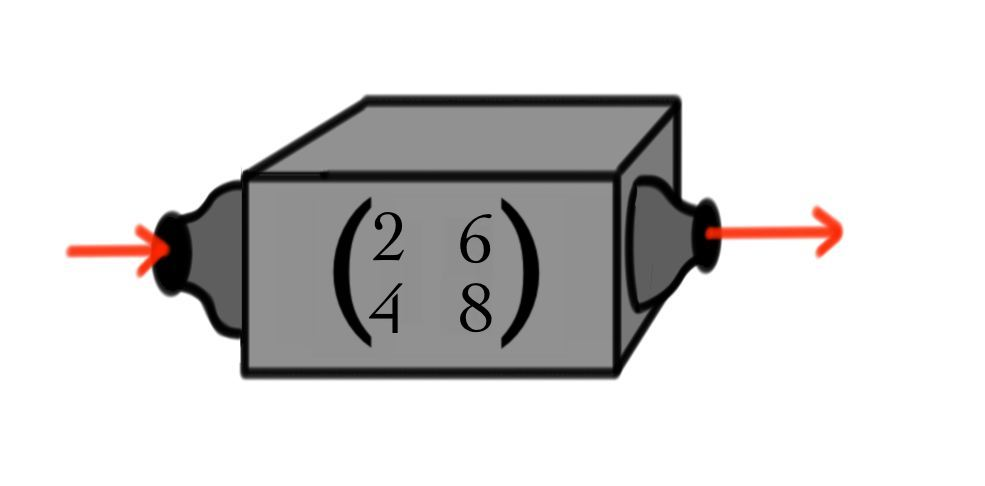
\includegraphics[scale=.15]{\whatIsPath//machine_matrix.jpg} }\!\!\!\!\!\!\colvec{2x+6y\\4x+8y}\, .
\]
Our fruity problem is now rather concise.
\begin{example}  (This time in purely mathematical language): \\[.2cm]
What vector~$  \colvec{x \\ y}$ satisfies 
$
    \begin{pmatrix}
      2     & 6 \\
      4     & 8
    \end{pmatrix}
  \colvec{x \\ y}
  =   \colvec{20 \\ 28}
$?
\end{example}
%\\
This is of the same~$Lv=w$ form as our opening examples. 
The matrix encodes fruit per container. The equation is roughly fruit per container times number of containers equals fruit. To solve for number of containers we want to \hypertarget{ch1divide}{somehow ``divide''} by the matrix. 


Another way to think about the above example is to remember the rule for multiplying a matrix times a vector.
\hypertarget{system2matrix}{If} you have forgotten this, you can actually  guess a good rule by making sure the matrix equation is the same as the system of linear equations.
This would require that
\[
 \begin{pmatrix}
      2     & 6 \\
      4     & 8
    \end{pmatrix}
  \colvec{x \\ y}
  :=   \colvec{2x+6y \\ 4x+8y}
\]
Indeed this is an example of
\hypertarget{ch1vecmult}{the general rule} that you have probably seen before
%\begin{center}
%``Turn the vector sideways, and combine it with the rows of the matrix" \end{center}
\begin{equation*}\label{2x2multiplication}
    \begin{pmatrix}
      p     & q  \\
      r      & s
    \end{pmatrix}
  \colvec{x \\ y}
  :=
  \colvec{px+qy \\ rx+sy}=x\colvec{p\\r} + y\colvec{q\\s}\, .
\end{equation*}
Notice, that the second way of writing the output on the right hand side of this equation is very useful because it
tells us what all possible outputs a matrix times a vector look like -- they are just sums of the columns of the matrix
multiplied by scalars. The set of all possible outputs of a matrix times a vector is called 
the {\bfseries column space}\index{Column Space!concept of} (it is also the image of the linear function defined by the matrix).
%\reading{1}{2}
\Reading{WhatIsLinearAlgebra}{2}


 


\noindent
Multiplication by 
\hypertarget{earlier}{a matrix} is an example of a \emph{Linear Function}\index{Linear Transformation!concept of}, because it takes one vector and turns it into another in a ``linear'' way.
Of course, we can have much larger matrices if our system has more variables.

\videoscriptlink{what_is_linear_algebra_Possibilities.mp4}{Matrices in Space!}{script_what_is_linear_algebra_hint}

\noindent
Thus
\hypertarget{Matrices are linear operators}{matrices can be viewed as linear functions.} 
The statement of this for the matrix in our fruity example is as follows.
\begin{enumerate}
\item\label{ITEM1}~$\begin{pmatrix}
      2             &6 \\
      4            &8
    \end{pmatrix}
   \lambda \colvec{x \\ y} 
   =\lambda  \begin{pmatrix}
      2             &6 \\
      4            &8
    \end{pmatrix}
   \colvec{x \\ y} ~$ and
\item\label{ITEM2}
$     \begin{pmatrix}
      2             &6 \\
      4            &8
    \end{pmatrix}
   \left[ \colvec{x \\ y} +\colvec{x' \\ y'} \right] 
   = \begin{pmatrix}
      2             &6 \\
      4            &8
    \end{pmatrix}
\colvec{x \\ y}
   +
    \begin{pmatrix}
      2             &6 \\
      4            &8
    \end{pmatrix}
    \colvec{x' \\ y'}
.$
\end{enumerate}
These equalities can be verified using the rules we introduced so far.
\begin{example} Verify that 
$\begin{pmatrix}
      2             &6 \\
      4            &8
    \end{pmatrix}$
is a linear operator.

\noindent
The matrix-function is homogeneous if the expressions on the left hand side and right hand side of the equation in part~\ref{ITEM1} above are indeed equal. 
\begin{equation*}
\begin{split}
\begin{pmatrix}
      2             &6 \\
      4            &8
    \end{pmatrix}
    \left[
   \lambda \colvec{a \\ b} \right]
 =
\begin{pmatrix}
      2             &6 \\
      4            &8
    \end{pmatrix}
   \colvec{\lambda a \\ \lambda b} 
 &=
  \lambda a \colvec{2 \\ 4} 
+   
     \lambda b \colvec{6 \\ 8} \\[2mm]&
 = \colvec{2\lambda a \\ 4\lambda a} 
+   
      \colvec{6\lambda b \\ 8\lambda b}=  \underline{\colvec{2\lambda a+6\lambda b\\4\lambda a+8\lambda b}} \end{split}\end{equation*}
while
 \begin{equation*}\begin{split} \lambda  \begin{pmatrix}
      2             &6 \\
      4            &8
    \end{pmatrix}
   \colvec{a \\ b} ~
   =
     \lambda\left[ a \colvec{2 \\ 4} 
+   
     b \colvec{6 \\ 8} \right]
   &=\lambda\left[\colvec{2a\\4a}+\colvec{6b\\8b}\right]\\[2mm]&=\lambda\colvec{2a+6b\\4a+8b} =  \underline{\colvec{2\lambda a+6\lambda b\\4\lambda a+8\lambda b} .}
     \end{split}\end{equation*}
\vspace{3mm}
\noindent
The underlined expressions are  identical, so the matrix is homogeneous. \\

The matrix-function is additive if the left and right side of the equation  in part~\ref{ITEM2} above are indeed equal. 

\begin{equation*}
\begin{split}
     \begin{pmatrix}
      2             &6 \\
      4            &8
    \end{pmatrix}
   \left[ \colvec{a \\ b} +\colvec{c \\ d} \right] 
   &= 
        \begin{pmatrix}
      2             &6 \\
      4            &8
    \end{pmatrix}
    \colvec{a +c\\ b+d}  
   =
        (a+c) \colvec{2 \\ 4} 
        +
         (b+d) \colvec{6 \\ 8}\\[2mm]&
         =
        \colvec{2(a+c) \\ 4(a+c)} 
        +
        \colvec{6(b+d) \\ 8(b+d)}
             =
       \underline{ \colvec{2a+2c +6b+6d\\ 4a+4c+8b+8d} }
       \end{split}\end{equation*}
 which we need to compare to  
\begin{equation*}
\begin{split}
  \begin{pmatrix}
      2             &6 \\
      4            &8
    \end{pmatrix}
\colvec{a \\ b}
 &  +
    \begin{pmatrix}
      2             &6 \\
      4            &8
    \end{pmatrix}
    \colvec{c \\ d}
=
a\colvec{2\\4} + b\colvec{6\\ 8} + c\colvec{2\\4} +d\colvec{6\\8}\\[2mm]&
=\colvec{2a\\4a} + \colvec{6b\\ 8b} + \colvec{2c\\4c} +\colvec{6d\\8d}
=\underline{\colvec{2a+2c +6b+6d\\ 4a+4c+8b+8d} }\, .
\end{split}\end{equation*}
Thus multiplication by a  matrix is additive and homogeneous, and so it is, by definition, linear. 
\end{example}

%\noindent

We have come full circle; matrices are just examples of the kinds of linear operators that appear in algebra problems like those in 
section~\ref{LTs}. 
Any equation of the form~$Mv=w$ with~$M$ a matrix, and~$v,w$ $n$-vectors is called  a {\itshape matrix equation}\index{Matrix equation}. 
Chapter~\ref{systems} is about efficiently solving systems of linear equations, or equivalently matrix equations.

\subsection{Matrix Multiplication is Composition of Functions}

What would happen if we placed two of our expensive machines end to end?
\[
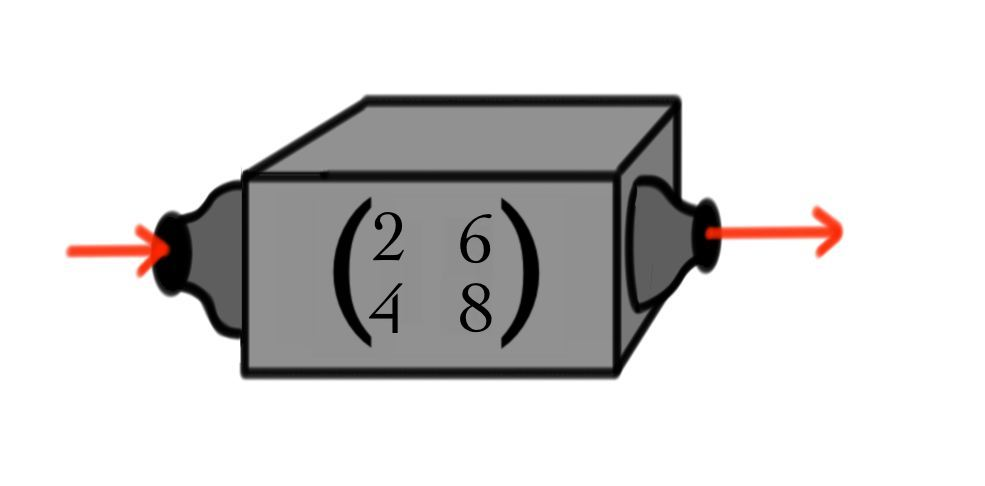
\includegraphics[scale=.15]{\whatIsPath//machine_matrix.jpg} \raisebox{1mm}{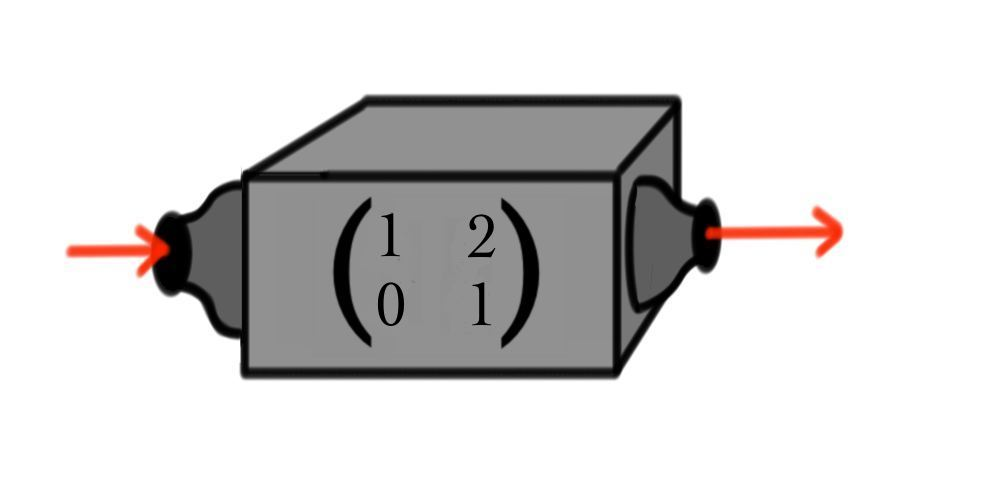
\includegraphics[scale=.15]{\whatIsPath//machine_matrix1.jpg}} \raisebox{12mm}{\Huge ?}
\]
The output of the first machine would be fed into the second. 
\[
\scalebox{.7}{$\colvec{x\\y}$}\hspace{-.6mm}\raisebox{-9mm}{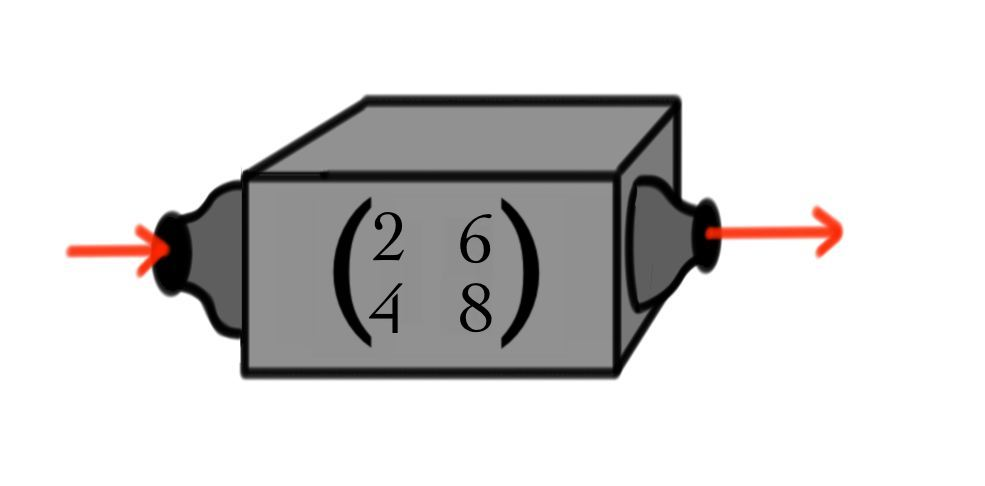
\includegraphics[scale=.12]{\whatIsPath//machine_matrix.jpg} }\!\!\!\!\!\!\scalebox{.7}{$\colvec{2x+6y\\4x+8y}$}
\raisebox{-9mm}{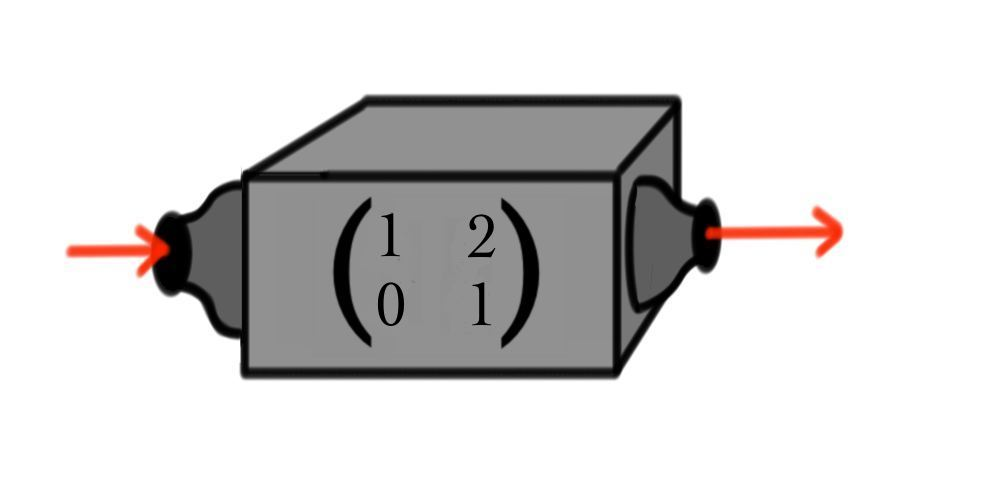
\includegraphics[scale=.12]{\whatIsPath//machine_matrix1.jpg} }\!\!\!\!\!\!\!\!\!\!\!\!\!
  \raisebox{-3mm}{ \scalebox{.7}{$\begin{array}{l}\ \ \ \ \colvec{1.(2x+6y)+2.(4x+8y)\\0.(2x+6y)+1.(4x+8y)}\\[4mm] \ =\colvec{10x+22y\\4x+8y}\end{array}$}}
\]
Notice that the same final result could be achieved with a single machine:
\[
\colvec{x\\y}\raisebox{-11mm}{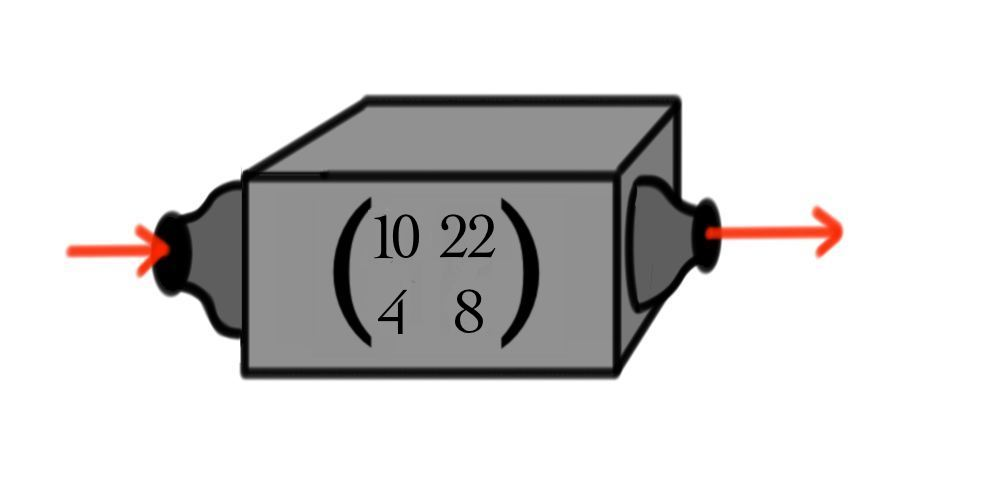
\includegraphics[scale=.15]{\whatIsPath//machine_matrix2.jpg} }\!\!\!\!\!\!\colvec{10x+22y\\4x+8y}\, .
\]
There is a simple matrix notation for this called {\itshape matrix multiplication}\index{Matrix multiplication}
\[
\begin{pmatrix}1&2\\0&1\end{pmatrix}
\begin{pmatrix}2&6\\4&8\end{pmatrix}
=\begin{pmatrix}10&22\\4&8\end{pmatrix}\, .
\] 
Try review problem~\ref{matmult} to learn more about matrix multiplication. 

In the language\footnote{The notation $h:A\to B$ means that $h$ is a function with domain $A$ and codomain $B$. See the webwork  background  set\hwref{Background}{3} if you are unfamiliar with this notation or these terms.} 
of functions, if \[f:U\longrightarrow V\quad \mbox{and}\quad g:V\longrightarrow W\]
the new function obtained by plugging the outputs if $f$ into $g$ is called $g\circ f$,
\[
g\circ f:
U\longrightarrow  W\]
where
\[
(g\circ f)(u)=g(f(u))\, .
\]
This is called the {\itshape composition of functions}\index{Composition of functions}.
Matrix multiplication is the tool required for computing the composition of linear functions.


\subsection{The Matrix Detour}
Linear algebra is about linear functions, not matrices. 
%This lesson is hard to learn after a full term of working with matrices. 
%Start thinking about this on day one of the course. 
The following presentation is meant to get you thinking about this idea constantly throughout the course.
\begin{center}
\shabox{Matrices only get involved in linear algebra when certain notational choices are made.}
\end{center}
To exemplify, lets look at the derivative operator again.

\begin{example}{of how matrices come into linear algebra.}\\
Consider the equation
%question ``which quadratic function $f$ satisfies
\[\left( \frac{d}{dx}+2\right) f= x+1\]
where $f$ is unknown (the place where solutions should go) and  the linear differential operator $\frac{d}{dx}+2$ is understood to take in quadratic functions (of the form $ax^2+bx+c$) and give out other quadratic functions. 

Let's simplify the way we denote the quadratic functions; 
we will  
\[{\rm denote~~}ax^2+bx+c \text{~~as~~} \colvec{a\\b\\c}_B.\]
The subscript $B$ serves to remind us of our particular notational convention; we will compare to another notational convention later. With the convention $B$ we can say
\begin{gather*}  \left( \frac{d}{dx}+2\right) \colvec{a\\b\\c}_B
=\left( \frac{d}{dx}+2\right)(ax^2+bx+c)\\
=(2ax+b)+(2ax^2+2bx+2c) = 2a x^2+(2a+2b)x+(b+2c)
\\
=\colvec{\mc{2a}\\2a+2b\\\mc{b+2c}}_B
= 
\left[ 
\begin{pmatrix}   
2&0&0\\
2&2&0\\
0&1&2
\end{pmatrix}
\colvec{a\\b\\c}\right]_B.
\end{gather*}
That is, our notational convention for quadratic functions has induced a notation for the differential operator $\frac{d}{dx}+2$ as a matrix. 
We can use this notation to change the way that 
the following two equations say exactly the same thing.
\[
 \left( \frac{d}{dx}+2\right) f=x+1
 \Leftrightarrow
\left[ 
\begin{pmatrix}   
2&0&0\\
2&2&0\\
0&1&2
\end{pmatrix}
\colvec{a\\b\\c}\right]_B = \colvec{0\\1\\1}_B.\]
Our notational convention has served as an organizing principle to yield the system of equations 
\[
\begin{array}{cc}
2a&=0\\
2a+2b&=1\\
b+2c&=1
\end{array}
\]
with solution $\colvec{0\\ \frac12\\[1mm] \frac14}_{\!B}  $, where the subscript $B$ is used to remind us that this stack of numbers  encodes the vector $\frac12x+\frac14$, which is indeed the  solution to our equation since, substituting for $f$ yields the true statement $\left(\frac{d}{dx}+2\right)(\frac12x+\frac14)=x+1$. 
\end{example}

It would be nice  to have a systematic way
to rewrite any linear equation as an equivalent matrix equation. 
It will be a little while before we can learn to  organize information in a way generalizable to all linear equations, 
but keep this example in mind throughout the course. 

The general idea is presented in the picture below; sometimes a linear equation is too hard to solve as is, but by organizing information and reformulating the equation as a matrix equation the process of finding solutions becomes tractable. 
\begin{center}
{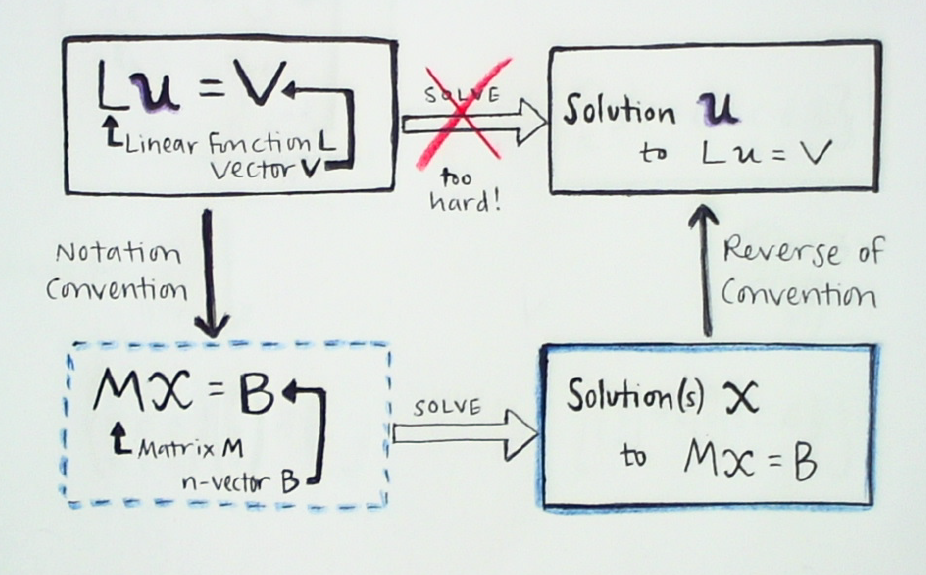
\includegraphics[width=.8\textwidth]{\whatIsPath/detourAbs} }\\
\end{center}
A simple example with the knowns ($L$ and $V$ are $\frac{d}{dx}$ and $3$, respectively) is shown below, although the detour is unnecessary in this case since you know how to anti-differentiate.
\begin{center}
{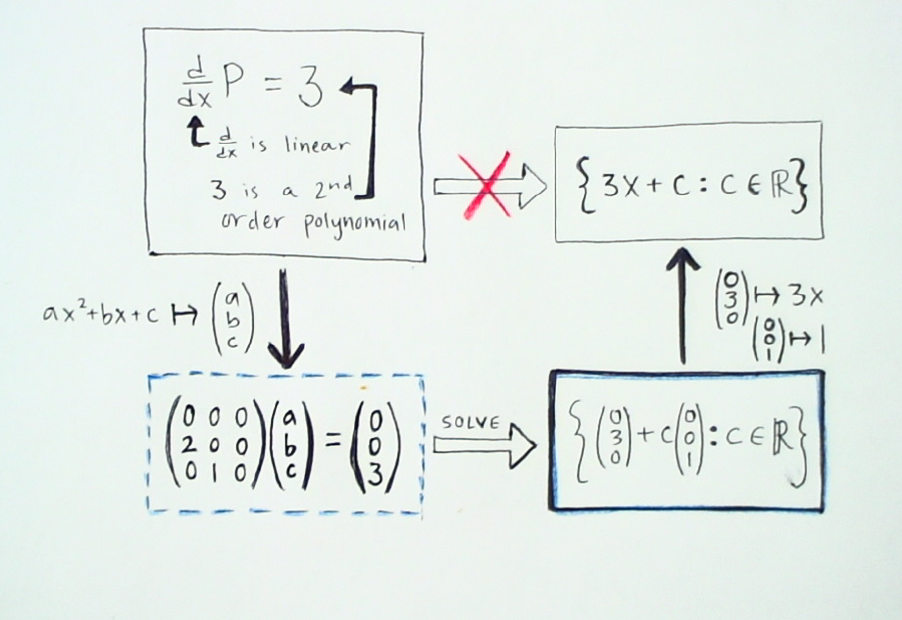
\includegraphics[width=.8\textwidth]{\whatIsPath/detourEg} }\\
\end{center}


To drive home the point that we are not studying matrices but rather linear functions, and that those linear functions can be represented as matrices under certain notational conventions, 
consider how changeable the notational conventions are. 


\begin{example}{of how a different matrix comes into the same linear algebra problem.}\\

\noindent Another possible notational convention  is to
\[\text{denote~~}a+bx+cx^2 \text{~~as~~} \colvec{a\\b\\c}_{\!\!\!B'}.\]
With this alternative notation
\begin{gather*}  \left( \frac{d}{dx}+2\right) \colvec{a\\b\\c}_{B'}
=\left( \frac{d}{dx}+2\right)(a+bx+cx^2)\\
=(b+2cx)+(2a +2bx+2cx^2 ) = (2a+b) + (2b+2c)x+2cx^2
\\
=\ccolvec{2a+b\\2b+2c\\2c}_{B'}
= 
\left[ 
\begin{pmatrix}   
2&1&0\\
0&2&2\\
0&0&2
\end{pmatrix}
\colvec{a\\b\\c}\right]_{B'}.\end{gather*}
Notice that we have obtained {\itshape a different matrix for the same linear function}. 
The  equation we started with 
\begin{gather*}
 \left( \frac{d}{dx}+2\right) f=x+1
 \Leftrightarrow
\left[ 
\begin{pmatrix}   
2&1&0\\
0&2&2\\
0&0&2
\end{pmatrix}
\colvec{a\\b\\c}\right]_{B'} = \colvec{1\\1\\0}_{\!B'}\\
\Leftrightarrow
\begin{array}{r}
2a+b=1\\
2b+2c=1\\
2c=0
\end{array}
\end{gather*}
has the solution 
$\colvec{ \frac14\\[1mm] \frac12\\[1mm]0}$. Notice that we have obtained {\itshape a different 3-vector for the same vector},  since in the notational convention $B'$ this 3-vector represents $\frac14+\frac12x$. 
\end{example}

One linear function can be represented (denoted) by a huge variety of matrices. %with the same effects for any choice of representation. 
The representation only depends on how vectors are denoted as n-vectors.


%We hope this helps you understand why we will be looking at matrices so much even though they will not be our primary objects of study. But, unfortunately we can not start at the climax of our story; 
%we must cover how to use matrices per se before we cover how to change to matrix notation and then use matrices! Thus, the next chapter is devoted to the study of matrices in and of them selves. 



%\section{Where are we going?}
%
%Let us reiterate, linear algebra is about more than just matrices. It is about linear operators. 
%While matrices are among the simplest linear operators, they are the most powerful; as hinted at above, complicated and confusing operators can be re-written as matrices as long as they are linear. Before one can see that, one must have a deep understanding of matrices and their structure. This course is mostly about learning that structure.
%
%To hint at what we meant by ``structure of matrices" lets look back on some math you already know.  
%The fundamental theorem of arithmetic says that any integer can be factored into a product of prime numbers (and bio further). 
%The fundamental theorem of algebra says that polynomials over the complex numbers can be factored into first order polynomials (and no further, e.g.~$x^4-1=(x+1)(x-1)(x+1)(x-1)$). 
%The prime numbers are the building blocks of integers and the first order polynomials are the building blocks of polynomials. We will first work toward answering the question, what are the building blocks of matrices? We will discover in chapter 2 that the building blocks are objects called elementary row operations. In Chapter 3 will categorize these objects in detail.

%This example uses augmented matrices which have not been introduced yet!
%\videoscriptlink{what_is_linear_algebra_3_3_matrix.mp4}{A~$3 \times 3$ matrix example}{scripts_what_is_linear_algebra_3_3_matrix}

%This vid uses the old first page of the text and  might be a bit confusing. 
%\videoscriptlink{what_is_linear_algebra_overview.mp4}{Video Overview}{video_what_is_overview}

%I've opted to use the word operator instead of transformation-David
%The matrix is an example of a \emph{Linear Transformation}\index{Linear Transformation!concept of}, because it takes one vector and turns it into another in a linear way:


%\References{
%Hefferon, Chapter One, Section 1\\
%Beezer, Chapter SLE, Sections WILA and SSLE\\
%Wikipedia, \href{http://en.wikipedia.org/wiki/System_of_linear_equations}{Systems of Linear Equations}
%}


\section{Review Problems}

You probably have already noticed that understanding sets, functions and basic logical operations 
is a must to do well in linear algebra. Brush up on these skills by trying these background webwork
problems:

\begin{center}
\begin{tabular}{|c|c|}
\hline
Logic &
\hwref{Background}{1}\\ 
Sets &
\hwref{Background}{2}\\ 
Functions &
\hwref{Background}{3}\\ 
Equivalence Relations &
\hwref{Background}{4}\\ 
Proofs &
\hwref{Background}{5}\\ 
\hline
\end{tabular}
\end{center}

\noindent
Each chapter also has reading and skills WeBWorK problems:
\vspace{2mm}

{\bfseries Webwork:} 
\begin{tabular}{|c|c|}
\hline
Reading problems &
\hwrref{WhatIsLinearAlgebra}{1}, \hwrref{WhatIsLinearAlgebra}{2}\\
\hline
\end{tabular}
\vspace{4mm}

\noindent
Probably you will spend most of your time on the following review questions:





\begin{enumerate}
\item \label{det33} Let $M=\begin{pmatrix}
m^1_1 & m^1_2 & m^1_3\\
m^2_1 & m^2_2 & m^2_3\\
m^3_1 & m^3_2 & m^3_3\\
\end{pmatrix}$.  Use row operations to put $M$ into \emph{row echelon form}.  For simplicity, assume that $m_1^1\neq 0 \neq m^1_1m^2_2-m^2_1m^1_2$.

Prove that $M$ is non-singular if and only if:
\[
m^1_1m^2_2m^3_3 
- m^1_1m^2_3m^3_2 
+ m^1_2m^2_3m^3_1 
- m^1_2m^2_1m^3_3 
+ m^1_3m^2_1m^3_2
- m^1_3m^2_2m^3_1
\neq 0
\]

\phantomnewpage

\item 
\begin{enumerate}
\item What does the matrix $E^1_2=\begin{pmatrix}
0 & 1 \\
1 & 0
\end{pmatrix}$ do to $M=\begin{pmatrix}
a & b \\
d & c
\end{pmatrix}$ under left multiplication?  What about right multiplication?
\item Find elementary matrices $R^1(\lambda)$ and $R^2(\lambda)$ that respectively multiply rows $1$ and $2$ of $M$ by $\lambda$ but otherwise leave $M$ the same under left multiplication.
\item Find a matrix $S^1_2(\lambda)$ that adds a multiple $\lambda$ of row $2$ to row $1$ under left multiplication.
\end{enumerate}

\phantomnewpage

\item Let $M$ be a matrix and $S^i_jM$ the same matrix with rows \(i\) and \(j\) switched.  Explain every line of the 
\hyperlink{rowswap}{series of equations} proving that $\det M = -\det (S^i_jM)$.

\phantomnewpage

%\item \label{prob_inversion_number} This problem is a ``hands-on'' look at why \hyperlink{permutation_parity}{the property} describing the parity of permutations is true.
%
%\hypertarget{inversion_number}{The \emph{inversion number}}\index{Permutation!Inversion number} of a permutation $\sigma$ is the number of pairs $i<j$ such that $\sigma(i)>\sigma(j)$; it's the number of ``numbers that appear left of smaller numbers'' in the permutation.  For example, for the permutation $\rho = [4,2,3,1]$, the inversion number is $5$. The number $4$ comes before $2,3,$ and $1$, and $2$ and $3$ both come before $1$.
%
%Given a permutation $\sigma$, we can make a new permutation $\tau_{i,j} \sigma$ by exchanging the $i$th and $j$th entries of $\sigma$.
%
%\begin{enumerate}
%\item What is the inversion number of the permutation \(\mu=[1,2,4,3]\) that exchanges 4 and 3 and leaves everything else alone? Is it an even or an odd permutation?
%
%\item What is the inversion number of the permutation \(\rho=[4,2,3,1]\) that exchanges 1 and 4 and leaves everything else alone? Is it an even or an odd permutation?
%
%\item What is the inversion number of the permutation \(\tau_{1,3} \mu\)? Compare the parity\footnote{The \emph{parity} of an integer refers to whether the integer is even or odd. Here the parity of a permutation $\mu$ refers to the parity of its inversion number.} of \(\mu\) to the parity of \(\tau_{1,3} \mu.\)
%
%\item What is the inversion number of the permutation \(\tau_{2,4} \rho\)? Compare the parity of \(\rho\) to the parity of \(\tau_{2,4} \rho.\)
%
%\item What is the inversion number of the permutation \(\tau_{3,4} \rho\)? Compare the parity of \(\rho\) to the parity of \(\tau_{3,4} \rho.\)
%\end{enumerate}
%
%\videoscriptlink{elementary_matrices_determinant_hint.mp4}{Problem~\ref{prob_inversion_number} hints}{scripts_elementary_matrices_determinants_hint}

\phantomnewpage

%\item \label{problem_permutation} (Extra credit) Here we will examine a (very) small set of the general properties about permutations and their applications. In particular, we will show that one way to compute the sign of a permutation is by finding the \hyperlink{inversion_number}{inversion number} $N$ of $\sigma$ and we have
%\[
%\sgn(\sigma) = (-1)^N.
%\]
%
%For this problem, let $\mu = [1,2,4,3]$.
%
%\begin{enumerate}
%\item Show that every permutation $\sigma$ can be sorted by only taking simple (adjacent) transpositions\index{Permutation!Simple transposition} $s_i$ where $s_i$ interchanges the numbers in position $i$ and $i+1$ of a permutation $\sigma$ (in our other notation $s_i = \tau_{i,i+1}$). For example $s_2 \mu = [1, 4, 2, 3]$, and to sort $\mu$ we have $s_3 \mu = [1, 2, 3, 4]$.
%
%\item \label{prob_part_relations} We can compose simple transpositions together to represent a permutation (note that the sequence of compositions is not unique), and these are associative, we have an identity (the trivial permutation where the list is in order or we do nothing on our list), and we have an inverse since it is clear that $s_i s_i \sigma = \sigma$. Thus permutations of $[n]$ under composition are an example of a \hyperref[groups]{group}. However note that not all simple transpositions commute with each other since
%\begin{align*}
%s_1 s_2 [1, 2, 3] & = s_1 [1, 3, 2] = [3, 1, 2]
%\\ s_2 s_1 [1, 2, 3] & = s_2 [2, 1, 3] = [2, 3, 1]
%\end{align*}
%(you will prove here when simple transpositions commute). When we consider our initial permutation to be the trivial permutation $e = [1, 2, \dotsc, n]$, we do not write it; for example $s_i \equiv s_i e$ and $\mu = s_3 \equiv s_3 e$. This is analogous to not writing 1 when multiplying. Show that $s_i s_i = e$ (in shorthand $s_i^2 = e$), $s_{i+1} s_i s_{i+1} = s_i s_{i+1} s_i$ for all $i$, and $s_i$ and $s_j$ commute for all $|i - j| \geq 2$.
%
%\item Show that every way of expressing $\sigma$ can be obtained from using the relations proved in part~\ref{prob_part_relations}. In other words, show that for any expression $w$ of simple transpositions representing the trivial permutation $e$, using the proved relations.
%
%\emph{Hint: Use induction on $n$. For the induction step, follow the path of the $(n+1)$-th strand by looking at $s_n s_{n-1} \cdots s_k s_{k\pm1} \cdots s_n$ and argue why you can write this as a subexpression for any expression of $e$. Consider using diagrams of these paths to help.}
%
%\item The simple transpositions \hyperlink{action}{acts on} an $n$-dimensional vector space $V$ by $s_i v = E^i_{i+1} v$ (where $E^i_j$ is \hyperlink{elem_matrix_row_swap}{an elementary matrix}) for all vectors $v \in V$. Therefore we can just represent a permutation $\sigma$ as the matrix $M_{\sigma}$\footnote{Often people will just use $\sigma$ for the matrix when the context is clear.}, and we have $\det(M_{s_i}) = \det(E^i_{i+1}) = -1$. Thus prove that $\det(M_{\sigma}) = (-1)^N$ where $N$ is a number of simple transpositions needed to represent $\sigma$ as a permutation. You can assume that $M_{s_i s_j} = M_{s_i} M_{s_j}$ (it is not hard to prove) and that $\det(A B) = \det(A) \det(B)$ \hyperref[detmultiplicative]{from Chapter~\ref*{elementarydeterminantsII}}.
%
%\emph{Hint: You to make sure $\det(M_{\sigma})$ is well-defined since there are infinite ways to represent $\sigma$ as simple transpositions.}
%
%\item Show that $s_{i+1} s_i s_{i+1} = \tau_{i, i+2}$, and so give one way of writing $\tau_{i, j}$ in terms of simple transpositions? Is $\tau_{i,j}$ an even or an odd permutation? What is $\det(M_{\tau_{i,j}})$? What is the inversion number of $\tau_{i,j}$?
%
%\item The minimal number of simple transpositions needed to express $\sigma$ is called the \emph{length}\index{Permutation!Length} of $\sigma$; for example the length of $\mu$ is 1 since $\mu = s_3$. Show that the length of $\sigma$ is equal to the inversion number of $\sigma$.
%
%\emph{Hint: Find an procedure which gives you a new permutation $\sigma^{\prime}$ where $\sigma = s_i \sigma^{\prime}$ for some $i$ and the inversion number for $\sigma^{\prime}$ is 1 less than the inversion number for $\sigma$.}
%
%\item Show that $(-1)^N = \sgn(\sigma) = \det(M_{\sigma})$, where $\sigma$ is a permutation with $N$ inversions. Note that this immediately implies that $\sgn(\sigma \rho) = \sgn(\sigma) \sgn(\rho)$ for any permutations $\sigma$ and $\rho$.
%\end{enumerate}

\item Let $M'$ be the matrix obtained from $M$ by swapping two columns $i$ and $j$. Show that $\det M'=-\det M $.

\item The scalar triple product of three vectors $u,v,w$ from $\Re^3$ is $u\cdot(v\times w)$. Show that this product is the same as the determinant of the matrix whose columns are $u,v,w$ (in that order). What happens to the scalar triple product when the factors are permuted? 

\item Show that if $M$ is a $3\times 3$ matrix whose third row is a sum of multiples of the other rows ($R_3=aR_2+bR_1$) then $\det M=0$. Show that the same is true if one of the columns is a sum of multiples of the others. 

\end{enumerate}

\phantomnewpage

%\newpage

%\begin{comment}
%There are two things to notice about  this list: First,  the range of operations in algebra seems to go beyond addition, subtraction, multiplication, and division while the range of possible objects goes beyond numbers. [In fact, its best to think of the objects (numbers) being generalized while trying to maintain
%the basic properties of addition, subtraction, {\itshape etc}..., as far as possible.]
%%; in fact, we mean only to hint at the variety of objects and operations found in algebra.   
%Second, these very different questions all have the same form. To emphasize this we restate them:
%\begin{example} (Algebra \hypertarget{AandD}{Questions} Restated)
%% Note to the Editor:
%% putting all in Ax=b is BAD! They emotionally want x to stand for a number, not a function,
%Solve
%\[
%{\cal A}\, {\bfseries x} = {\bfseries b}\, ,
%\]
%where
%\begin{enumext}[label=\Alph*,wrap-label=(#1)]
%\item \label{A}
%${\bfseries x}$ and ${\bfseries b}$ are numbers, \[{\cal A}\, {\bfseries x}:=10 \, {\bfseries x}\, ,\]
%and ${\bfseries b}=3$.
%%What 
%%number~$x$ satisfies~$Ax=10$ where~$Ax:=5x?$\\[-.6cm]
%\item 
%${\bfseries x}$ and ${\bfseries b}$ are 3-vectors,  \[{\cal A}\, {\bfseries x}:=\colvec{1 \\ 1\\ 0} \times {\bfseries x}\, ,\]\\
%\vspace{-15mm}
%and ${\bfseries b}=\colvec{1\\1\\0}$.
%%What vector~$v$ satisfies~$Bv = \colvec{0\\1\\1}$% \\
%%where ~$Bv:=\colvec{1 \\ 1\\ 0} \times v$?\\[-.4cm]
%\item 
%${\bfseries x}$ and ${\bfseries b}$ are polynomials in the variable $x$, \[{\cal A}\, p(x):=x\int_{-1}^1 yp(y)dy\, ,\] 
%and ${\bfseries b}=x$.
%%What polynomial~$g$ satisfies~$Cg=h$ where~$Cg$ is the function defined by \\[.3cm]
%%$Cg(x)=\int_{-1}^1 f(x,y)g(y) dy = h(x)$ where~$f(x,y):=xy,~h(x):=x$?\\[-.5cm]
%\item ${\bfseries x}$ and ${\bfseries b}$ are polynomials, 
%\[
%{\cal A}\,  p(x):=\frac{dp(x)}{dx}-2p(x)\, ,
%\]
%and ${\bfseries b}=0$
%%What polynomial~$f$ satisfies~$Df=0$ 
%%where~$Df$ is the function \\[.3cm]
%%$Df(x):=x\frac{d}{dx}f(x)-2f(x)$?\\[-5mm]
%\item  \label{E}
%${\bfseries x}$ and ${\bfseries b}$ are functions, 
%\[
%{\cal A}  \big(f(x) \big):= f''+f^3\, ,
%\]
%and ${\bfseries b}=\sqrt{x}$.
%%What function~$f$ satisfies~$Ef=g$ where~$Ef:=f''(x)+\big(f(x)\big)^3$ and~$g(x):=\sqrt{x}$?
%\end{enumext}
%\end{example}
%\noindent
%\reading{1}{1}
%You probably sense already that one of our main subjects will be the  study of equations 
%that can be written in the form
%\begin{center}
%\shabox{$Ax=b$}
%\end{center}
%%\begin{eqnarray*}
%%Ax=b
%%\end{eqnarray*}
%but where $x$ and $b$ can be much more general creatures than just numbers. The technical answer to the question ``how general?'',
%is that $x$ and $b$ will be {\itshape vectors}. We will say much more about what this means later, but for now all you need
%to know is that vectors are objects that you can {\itshape add} and {\itshape scalar multiply}, so that the algebraic operations
%\[
%x+x'\, ,\mbox{ and } c\, x\, ,
%\]
%where $c$ is any number, make sense.
%
%You might also be wondering why we wrote ${\cal A}\big(f(x)\big)$ rather than ${\cal A} f(x)$ in part~(\ref{E}) of our example,
%or perhaps why we did not write ${\cal A}({\bfseries x})$ in part~(\ref{A}). In fact all the the above problems involve functions (denoted ${\cal A}$)
%of vectors. However, in the first four examples the function~${\cal A}$ (that takes in a some sort of vector and returns a vector as its output)
%is a {\itshape linear operator} which means that it obeys a
%very special  property called {\itshape linearity}. This is the ``Linear'' in Linear Algebras and we will explain it next. 
%
%%%%%%%%%%%%%%%%%%%%%%%%%%%%%%%%%%%%%
%
%
%%\newpage
%\section{Operators: Functions of Functions}
%A few comments on jargon and notation are in order before we move on. ~$D$ takes in functions like~$x^4$ and gives out functions like~$4x^4-2x^4=2x^4$. You could say that~$D$ is a function that takes in functions and gives out functions.  
%Alternatively, that awful combination of words can be avoided by using the word 
%``{\itshape operator}" instead of ``function";
%~$D$ is an operator that takes in functions and gives out functions. 
% Similarly,~$C$ is an operator that takes in, for example,~$x^3$ and gives out ~$\frac12 x$. 
%We hope you can understand why we don't always use the 
%parentheses notation for arguments of functions when we think of the function as an operator;~$Dg(x)$ looks much better~$D(g)(x)$.
%
%%Video of operators? 
%
%If we are going to think of~$B$ as an operator too we need to understand the objects it takes in and gives out in a new way.
%It takes vectors from 3-space to vectors in 3-space. 
%Such vectors  
%\hypertarget{vecs as fun}{are really functions;} 
%a vector from 3-space~$v$ is a function whose domain is just (the set containing only)~$1,2,$ and~$3$. 
%
%
%\begin{example}
%\noindent
%The vector~$v=\colvec{v_1\\v_2\\v_3}=\colvec{7\\14\\21}$ is the function that: \\[.4cm]
%\begin{center}
%\begin{tabular}{l}
%Takes in~$1$ and gives out~$v_1=7$\\[1mm]
%Takes in~$2$ and gives out~$v_2=14$\\[1mm]
%Takes in~$3$ and gives out~$v_3=21$.\\[1mm]
%\end{tabular}
%\end{center}
%\end{example}
%
%\noindent
%This is an explicit definition of a function as opposed to of the more familiar algebraic definition. In analogy to defining a function~$f$ with domain all real numbers by the algebraic statement~$f(x)=7x$, we can define the function~$v$ by~$v_i=7i$. 
%The operator~$B$ takes in such a  function and gives out another. For example~\[Bv=\colvec{1\\1\\0}\times \colvec{7\\14\\21}=\colvec{21\\-21\\7}.\]
%
%
%You can also think of vectors from two space as functions with domain (the set containing only)~$1$ and~$2$. Similarly vectors from n-space are functions of (the set containing only)~$1,2,...,n$. This includes the case~$n=1$; we can even think of~$A$ as an operator. 
%
%\reading{1}{2}
%
%
%
%Digest what you can of these ideas now, but don't worry if you feel that some of this new stuff is not sinking in immediately. We will revisit all of these ideas. The point here is not to learn about any of the particular operators~$A,B,C,D,E$ but rather to show you that the world of algebra is much bigger than the study of questions involving just exponentiation, multiplication, division, addition and subtraction of numbers. Let your imagination go wild with our examples as inspiration. Imagine all the possible integral operators like~$C$ and differential operators like~$D$. We hope you will conclude that your adventures in algebra are just beginning, and that there are many very difficult problems out there. 
%The tools you will learn in linear algebra will help you answer all four of these example questions in an efficient way with the same method. That is the long story we wish to tell. 
%\end{comment}
%
%%<picture please: flow chart with algebra problem-> linear or not linear, if linear then-> matrix equation
%
%%\newpage
%%%%%%%%%%%%%%%%%%%%%%%%%%%%%%%%%%%
%%%%%%%%%%%%%%%%%%%%%%%%%%%%%%%%%%%
%
%
%\section{What is Linear?} 
%
%\begin{example} (Vectors) \\[-.5cm]
%\begin{enumext}[label=\Alph*,wrap-label=(#1)]
%\item Numbers. If
%\item What vector~$v$ from 3 space satisfies the cross product equation~$ \colvec{1 \\ 1\\ 0} \times v = \colvec{0\\1\\1}$?\\[-.4cm]
%\item What polynomial~$g$ satisfies~$\int_{-1}^1 f(x,y)g(y) dy = h(x)$, \\[.2cm]
% where~$f(x,y):=xy$ and~$h(x):=x$?\\[-.5cm]
%\item What power series~$f$ satisfies~$x\frac{d}{dx} f(x) -2f(x)=0$?
%%\item What power series~$f$ satisfies~$x\frac{d}{dx} f(x) -2f(x)=0$?
%\item What what function~$f$ satisfies~$f''(x)+f^3(x) =\sqrt{x}~$?
%\end{enumext}
%\end{example}
%
%
%
%
%Students often ask questions like ``how do I know when to use a particular method"? A question like ``how do I know when to use integration by parts?" is hard to  answer, but in contrast, ``when can I use  linear algebra?" is easy to answer: %for the kinds of questions given above; 
%{\itshape when the operator involved is linear.} \\
%
%\noindent
%An operator~$E$ is \hypertarget{asked in chapter 1}{said to be linear} if it has two properties:\\[-.5cm]
%\begin{enumerate}
%\item {\itshape Homogeneity:} ``Constants can be pulled out"
%\[E(cv)=cEv\, .\] \\[-.5cm]
%\item {\itshape Additivity:} ``The operator can be distributed"
%\[E(v+u)=Ev+Eu\, .\] 
%\end{enumerate}
%
%
%
%
%\noindent
%A great example is the derivative operator: for any two functions~$f$,~$g$ and any number~$c$ the derivative operator satisfies\\[-.5cm]
%\begin{example} (The derivative operator is linear)\\
%\begin{enumerate}
%\item ~$\frac{d}{dx} (cf)=c\frac{d}{dx} f$, \\[-.5cm]
%\item~$\frac{d}{dx}(f+g)=\frac{d}{dx}f+\frac{d}{dx}g$.\\[-.5cm]
%\end{enumerate}
%\end{example}
%\noindent
%We now explicitly verify that~$B$ and~$C$ are linear. You will verify that~$A$ and~$D$ are linear in the \hyperlink{ch1probset}{problem set} that ends this chapter.  \\
%
%\begin{example} Verifying that~$B$ is linear:
%
%We need to check that $B$ is linear acting on any vector $v=\colvec{x\\ y\\ z}$ so we compute~$Bv$
%using the cross product
%\[
%Bv=\colvec{1 \\ 1\\ 0} \times \colvec{x \\ y\\ z}=\colvec{z\\ -z\\y-x}\, .
%\]
%Now, until we know what a scalar multiple $cv$ of the vector $v$ means, the problem makes no sense. 
%Here we make (the logical) choice
%\[
%c\colvec{x \\ y\\ z} := \colvec{cx\\ cy\\ cz}\, .
%\]
%Now, using this definition and our result for how $B$ acts on an arbitrary vector we find:
%\[
%B(cv)=B\colvec{cx\\ cy\\ cz}=\colvec{cz\\-cz\\cy-cx}\, .
%\]
%We hope that this coincides with $cBv$ which also compute using our result for $Bv$ and the definition
%for multiplying a vector by a number:
%\[
%cBv=c\colvec{z\\ -z\\y-x}=\colvec{cz\\ c(-z)\\c(y-x)}=\colvec{cz\\-cz\\cy-cx}\, .
%\]
%Thankfully, we got the same result for both $B(cv)$ and $cBv$, so the homogeneity property holds.
%
%We still have to check additivity. Again, this makes no sense until we define what the sum $v+u$ of two arbitrary vectors $v=\colvec{x\\y\\z}$ 
%and $u=\colvec{x'\\y'\\z'}$. For that we again make a logical choice
%\[
%\colvec{x\\y\\z}+\colvec{x'\\y'\\z'}:=\colvec{x+x'\\y+y'\\z+z'}\, .
%\]
%Again, we have to make two computations: $B(u+v)$ (first add then act with $B$) and $Bu+Bv$ (first act with $B$, then add):
%\begin{gather*}
%B(u+v)=B\colvec{x+x'\\y+y'\\z+z'}=\colvec{z+z'\\-(z+z')\\(y+y')-(x+x')}=\colvec{z+z'\\-z-z'\\y+y'-x-x'}\, ,
%\\
%Bu+Bv=B\colvec{x\\y\\z}+B\colvec{x'\\y'\\z'}=\colvec{z\\-z\\y-x}+\colvec{z'\\-z'\\y'-x'}=\colvec{z+z'\\-z-z'\\y+y'-x-x'}\, .
%\end{gather*}
%Both computations give the same answer so now we know that $B$ also obeys additivity and can conclude that $B$ is linear.
%%AI)~$A(cx)=5cx= c5x=cAx$, \\
%%AII) A(x+y)=5(x+y)=5x+5y=Ax+Ay\\
%%\item~$B(cv)=\colvec{1 \\ 1\\ 0} \times cv
%%\!\!\!\!\!\!\!\!\!\!\!\!\!\!\stackrel{\rm \begin{array}{c}\rm\scriptstyle Using\  the\ rule\\[-2mm] \rm\scriptstyle for\ cross\ products\ of\\[-2mm]\rm
%%\scriptstyle scalar\ multiples\\\downarrow\\[1mm]\end{array}}= 
%%\!\!\!\!\!\!\!\!\!\!\!\!\!\!c\colvec{1 \\ 1\\ 0} \times v=c\, Bv$\, .\\
%%\item~$B(u+v)=\colvec{1 \\ 1\\ 0} \times (u+v)
%%\!\!\!\!\!\!\!\!\!\!\!\!\!\!\stackrel{\rm \begin{array}{c}\rm\scriptstyle Using\  the\ rule\\[-2mm] \rm\scriptstyle for\ cross\ products\\[-2mm]\rm
%%\scriptstyle of\ sums\\\downarrow\\[1mm]\end{array}}
%%=\!\!\!\!\!\!\!\!\!\!\!\!\!\!\colvec{1 \\ 1\\ 0} \times u+\colvec{1 \\ 1\\ 0} \times v =Bu+Bv\, .$\\[.5cm]
%%\end{enumerate} 
%\end{example} 
%The above example looks a little silly, this because it is really just checking something you probably already know about cross products of vectors. Namely, if $u$, $v$ and $w$ are vectors and $c$ is a number then
%\[
%w\times(cv)=c(w\times v)\quad\mbox{and}\quad  w\times(v+u)=w\times v+w\times u\, .
%\]
%You might also have noticed how important it was to know what $cu$ and $u+v$ actually meant to even solve the problem.
%In fact, one of the reasons linear algebra is so powerful, is that it can be applied to any choice for what $cu$ and $u+v$ mean
%that happens to obey a few basic rules. You will learn about these in Chapter~\ref{\vectorSpacesPath}.
%
%Here is another example involving linear operators made from integrals where we assume all the usual rules for integrals. Notice how much easier checking linearity is.
%\begin{example} Verifying that~$C$ is linear:\
%\begin{enumerate}
%\item~$C(cg)(x)= \int_{-1}^1f(x,y) cg(y)dy =c\int_{-1}^1f(x,y) g(y)dy =c\,Cg(x)$\\[.2cm]
%\item~$C(g_1+g_2)(x) =  \int_{-1}^1f(x,y) [g_1(y)+g_2(y)]dy\\[.2cm]
%\phantom{a}~~~~~
%=
%\int_{-1}^1f(x,y) g_1(y)dy
%+\int_{-1}^1f(x,y)g_2(y)dy
%=(Cg_1 +Cg_2)(x)$\\%[.4cm]
%\end{enumerate}
%\end{example}
%%DI)~$D(cf)(x)=(x\frac{d}{dx}-2)cf(x)=c(x\frac{d}{dx}-2)f(x)=cDf(x)$\\[.1cm]
%%DII)~$D(f_1+f_2)(x)=xf_1'(x)-2f_1(x) +xf_2'(x)-2f_2(x) =(Df_1+Df_2)(x)$.\\
%%You now know how to test if an operator is linear, and have some examples.  
%\noindent 
%One moral of our story is that if~$A$ is a {\itshape linear} operator while~$b$ and~$x$ are vectors, then~$Ax=b$ is equivalent to a matrix{\itshape -type} equation. 
%That is why we will begin by studying matrices.\\
%% We have only hinted at the wide range of possible examples for linear operators.
%This moral does {\itshape not} apply to non-linear operators:
%\begin{example} Show that~$E$ is {\itshape not} linear.\\[-5mm]
%\begin{enumerate}  
%\item~$E(5f)=5f''+5^3f^3 \neq 5f''+5f^3=5Ef~$\\[-5mm]
%\item Not needed.%\\[-5mm]
%\end{enumerate}  
%The operator~$E$ is not linear because it is not homogeneous.\
%\end{example}
%
%Actually,~$E$ is not additive either, but we did not need to show this. Once either one of the linearity properties is broken, the operator is not linear. (Unfortunately, you are a criminal the moment that you break just one law, no matter if you are a law abiding citizen in every other way!)
%
%\videoscriptlink{Homnotadd.mp4}{A Homogeneous Nonlinear Operator}{scripts_H}
%
%\begin{example} Show that operator~$Y$ that acts on numbers by~$Yx=5x+3$ is not linear. \\ 
%Lets check additivity first:
%\[
%Y(x+y)= 5(x+y)+3=(5x+3)+(5x)\neq (5x+3)+(5x+3)=Yx+Yy\, .
%\]
%This proves linearity, unfortunately homogeneity fails:
%\[Y(cx)=5cx+3=c (5x+3) +3 -3c= c\, Yx +3-3c\neq cYx \mbox{ if } c\neq1\, .\]
%Notice that the special case $c=1$ holds (and just says $Y(1.x)=1.Yx$), but the homogeneity
%requirement must work for {\itshape any} $c$. 
%
%The operator~$Y$ is neither homogeneous nor additive, and therefore not linear.
%\end{example}
%
%This example might surprise you because the graph of the equation~$y=5x+3$ is a line, and what else could linear mean other than ``line-like"? In fact, there is a linear operator associated with this equation: 
%the operator~$L$ that acts on two-vectors as 
%\[L\colvec{x\\y}=y-5x.\] 
%The line is then the collection of solutions to 
%\[L\colvec{x\\y}=10 \Leftrightarrow y-5x=3 \,.\] 
%Similarly, the  operator~$M$ on 3-space with 
%\[M\colvec{x\\y\\z}=2x-3y+5z\] 
%is linear. The set of solutions to 
%\[M\colvec{x\\y\\z}=10 \Leftrightarrow 2x-3y+5z=10\] 
%form a plane. Lines and planes are {\itshape level sets} of linear functions. 
%
%\videoscriptlink{Linear_Operator_on_Lines.mp4}{Linear Operators Preserve Lines}{scripts_H}
%
%
%
%%It is one thing to be able to tell which operators are linear and which are not, and it is another to have a feel for what linear operators do. Lets look at three simple example problems to get a feel for this. On the way we will introduce the main tool of linear algebra, the idea of a matrix. \\
%
%%%%%%%%%%%%%%%%%%%%%%%%%%%%%%%%%%%%%%%%%%%%%
%%%%%%%%%%%%%%%%%%%%%%%%%%%%%%%%%%%%%%%%%%%%%
%
%\noindent
%
